\documentclass[11pt,a4paper,oneside,onecolumn,fleqn,dvipdfmx]{jsarticle}

\usepackage{preamble}

\usepackage{geometry}
\geometry{left=25mm,right=25mm,top=30mm,bottom=30mm}
\usepackage{caption}
\captionsetup[table]{labelsep=space}

\begin{document}

\thispagestyle{empty}
\begin{center}
    \vspace*{20pt}
    {\fontsize{50pt}{0pt}\selectfont{卒業論文中間報告書}}
    \vskip 60pt
    {\fontsize{32pt}{0pt}\selectfont{EVの駆動力制御のための\\[5pt]機械学習を用いた\\[5pt]路面$\mu -\lambda$曲線推定を伴う\\[5pt]最適スリップ率推定}}
    \vskip 60pt
    {\fontsize{32pt}{0pt}\selectfont{2026年10月02日 \ 提出}}
    \vskip 60pt
    {\fontsize{32pt}{0pt}\selectfont{指導教員}}
    \vskip 20pt
    {\fontsize{32pt}{0pt}\selectfont{藤本 博志 教授}}
    \vskip 60pt
    {\fontsize{32pt}{0pt}\selectfont{電気電子工学科}}
    \vskip 20pt
    {\fontsize{32pt}{0pt}\selectfont{03-250513\ \ 堀越太智}}
\end{center}
\clearpage

%==================================================
% 目次
%==================================================

\pagenumbering{roman}

\tableofcontents

\listoffigures

\listoftables
\clearpage

%==================================================
% 本文
%==================================================

\pagenumbering{arabic}
\setcounter{page}{1}


\section{序論}
\subsection{電気自動車の運動制御}
電気自動車(Electric Vehicle : EV)は, 走行時にCO$_2$を排出しないという特徴に加え, 電動モータを駆動源とするため内燃機関車と比較するとおよそ100倍の速さのトルク応答性を持つ他, 電流センサを用いて正確なトルク測定が可能であるという特徴がある\cite{yoshimura}. 

EVは主にオンボードモータ車(On-Board Motor EV : OBM-EV)とインホイールモータ車(In-Wheel Motor EV : IWM-EV)に分類される. 
特にIWM-EVはその名の通り各車輪のホイール部分にモータが分散配置されているため, 各輪を独立に制御できドライブシャフトの共振を排除できるという特徴がある. 
これらの特徴から, IWM-EVを対象とした運動制御に関する研究が盛んに行われており, その中の一つにタイヤから路面に伝達される駆動力を対象とする駆動力制御(Driving Force Control : DFC)がある\cite{binhminh}. 

\subsection{IWM-EVの駆動力制御}
駆動力制御は, Fig.\ref{fig:1_DFC_abs}に示すように, 車両運動制御の段階において, 各車輪の駆動力指令値$F_\mathrm{d}^*$が求められた後に働く下層の制御である.
IWM-EVにおいては、各車輪に対し独立に駆動力制御を行うことができる.
駆動力制御の出力は各車輪へのトルク指令値$T^*$である. 
ブロック線図をFig.\ref{fig:1_DFC_circuit}に示す. 駆動力制御はカスケード構造を取り, インナーループで車輪速制御(Wheel Speed Control : WSC)を行いアウターループにおいて駆動力$F_\mathrm{d}$を制御する.
また, 駆動力制御には操作量としてスリップ率を用いているが, その中でスリップ率リミッタなる機構が存在する. その機構が駆動力制御中の安定走行において重要な役割を果たしている. 詳細は後述する.

\subsection{駆動力$F_\mathrm{d}$と路面摩擦係数$\mu$, スリップ率$\lambda$}
タイヤ・路面間の前後方向駆動力$F_{\mathrm{d},ij}$は, 路面摩擦係数$\mu_{ij}$と垂直荷重$F_{z,ij}$を用いて
以下のように表される.
\begin{equation}
    \label{eq:1_Fd}
    F_{\mathrm{d},ij} = \mu_{ij} F_{z,ij}
\end{equation}
また, 路面摩擦係数$\mu$は, スリップ率$\lambda$と一定の関係性を持つことが一般に知られている. 
路面状態によりその$\mu-\lambda$特性は異なるが, 一般にはFig.\ref{fig:1_mu-lambda}に示すような低スリップ領域では線形, 高スリップ領域では非線形な関係性を示す. 
この曲線を一般に$\mu-\lambda$曲線という.


\subsection{駆動力制御とスリップ率リミッタ}
Fig.\ref{fig:1_mu-lambda}からわかるように, 一定以上のスリップ率となると路面摩擦係数$\mu$および駆動力$F_\mathrm{d}$は飽和し, グリップ力を失う. 
一方, 駆動力指令値$F_\mathrm{d}^*$は任意の値を取りうるため, ピーク摩擦係数$\mu_\mathrm{peak}$が小さく滑りやすい低$\mu$路においては, 物理的に駆動力指令値に追従できなくなるケースが存在する. 
この場合, 駆動力制御器は本来出力できない駆動力指令値に追従しようと, 車輪速およびトルク指令値を過大にしてしまう結果, 大空転を起こし走行状態が不安定になり, 乗り心地の悪化や車両の走行安定性低下のリスクが発生する. 
このリスクを防止するのがスリップ率リミッタ$\lambda_\mathrm{lim}$である. 
スリップ率リミッタによりスリップ率に上限を設けることで, グリップを失うリスクを抑えることができる. 

\subsection{最適スリップ率 $\lambda_{\mathrm{peak}}$}
従来の駆動力制御\cite{yoshimura}では, スリップ率リミッタ$\lambda_\mathrm{lim}$を一定の値に固定していた. 一方, 路面により$\mu-\lambda$曲線の形状は異なるため, 固定のスリップ率リミッタでは
本来出せる最大駆動力以下の出力しか出せない場合が存在してしまう. 
そこで, $\lambda_\mathrm{lim}$を, ピーク摩擦係数$\mu_{\mathrm{peak}}$に対応する最適スリップ率$\lambda_\mathrm{peak}$に設定することができれば, 走行安定性を保証しながらその路面で発揮しうる最大の駆動力を得ることができ, 望ましい.
一方で, 路面状態により$\mu-\lambda$特性は大きく異なり$\lambda_\mathrm{peak}$も逐次変化するため, これをリアルタイムに推定することは容易ではなく, この研究が盛んに行われている\cite{binhminh,zengin,morimoto,hannes}.

\begin{figure}[tb]
    \centering
    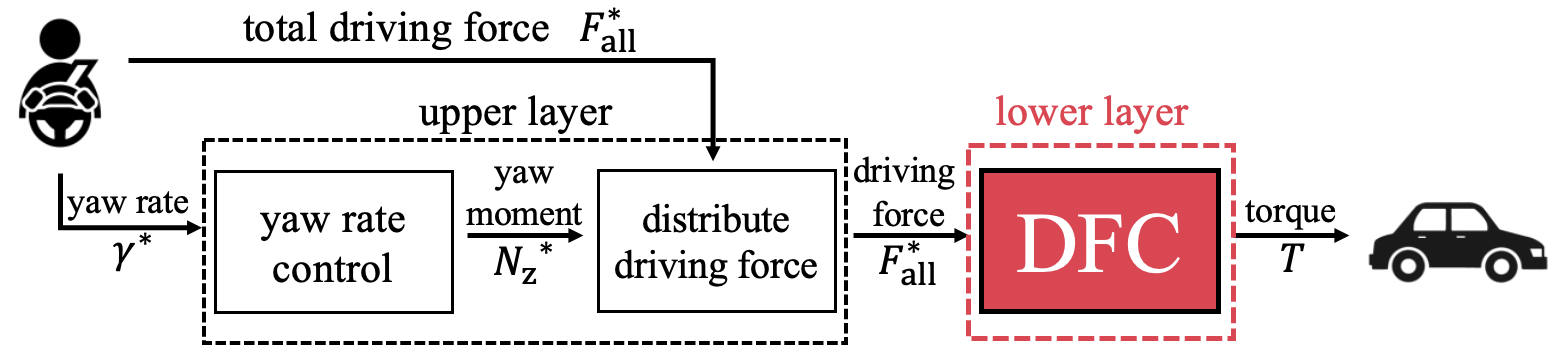
\includegraphics[width=1\linewidth]{fig/1_DFC_abs.png}
    \caption{駆動力制御(DFC)の運動制御に対する位置付け.}
    \label{fig:1_DFC_abs}
\end{figure}

\begin{figure}[tb]
    \centering
    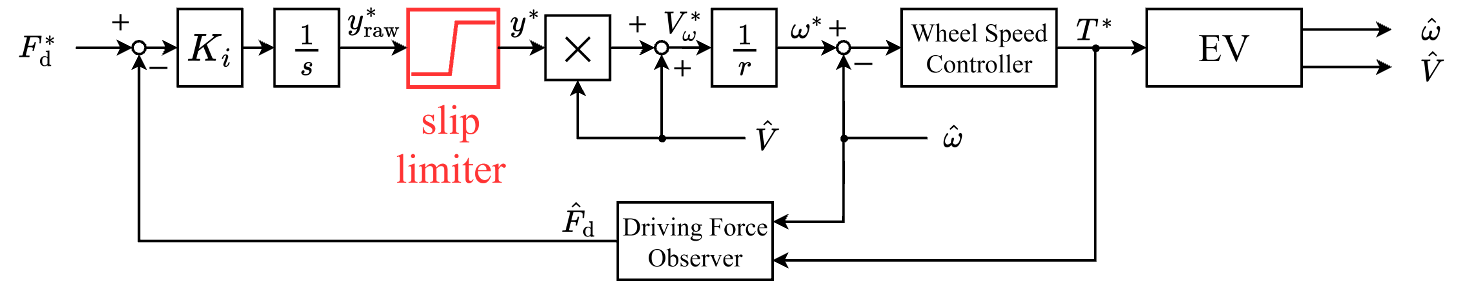
\includegraphics[width=1\linewidth]{fig/1_DFC_circuit.png}
    \caption{駆動力制御(DFC)のブロック線図.}
    \label{fig:1_DFC_circuit}
\end{figure}

\begin{figure}[tb]
    \centering
    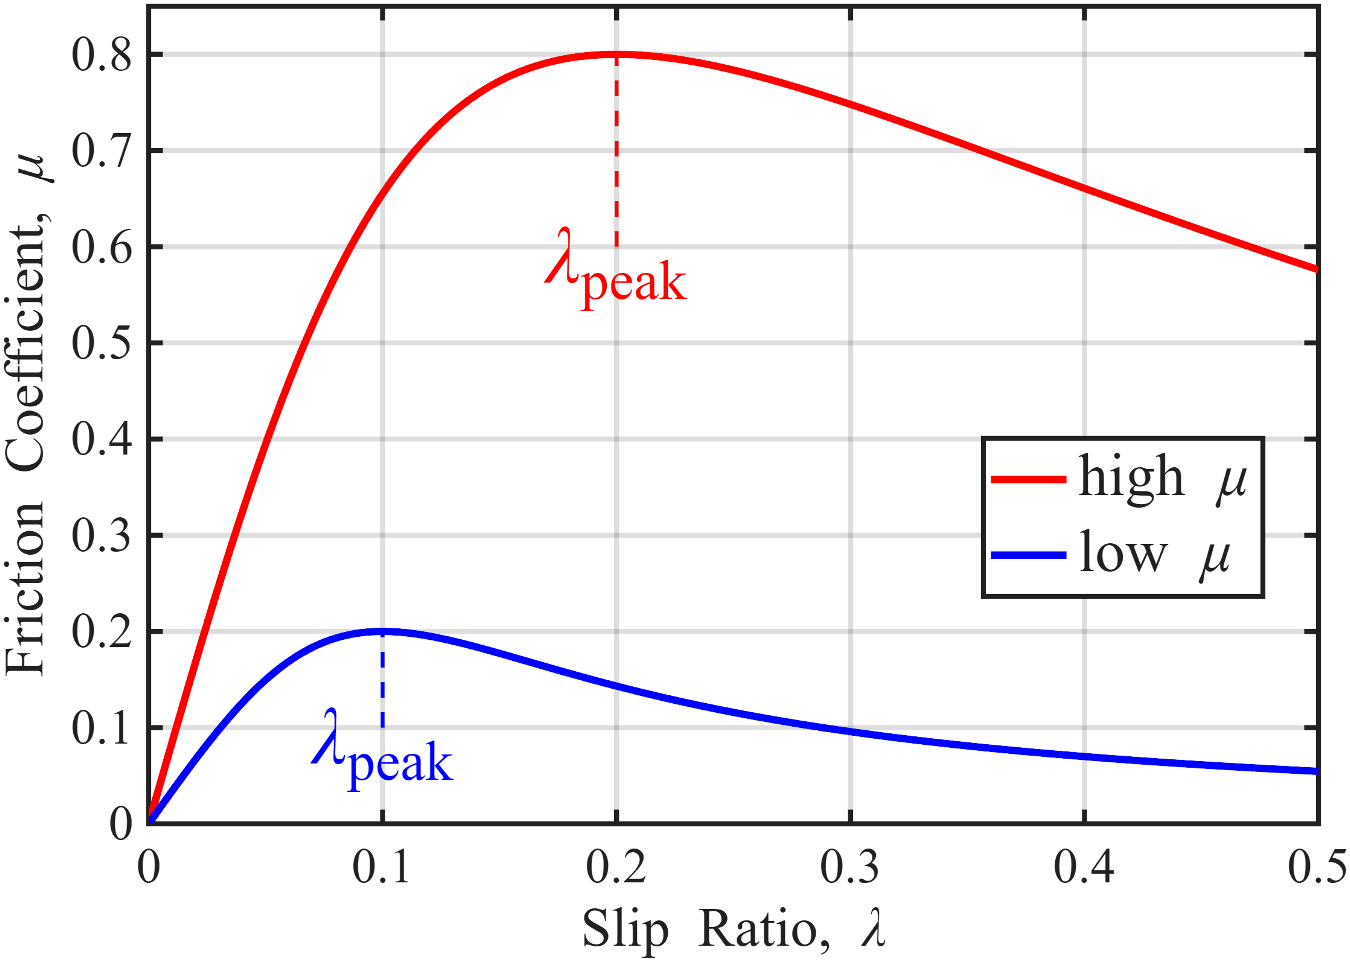
\includegraphics[width=0.6\linewidth]{fig/1_mu-lambda.png}
    \caption{$\mu-\lambda$曲線.}
    \label{fig:1_mu-lambda}
\end{figure}


\subsection{従来研究}
最適スリップ率推定の研究として, 逐次最小二乗法(Recursive Least Squares : RLS)に基づく極値探索アルゴリズムを用いた手法\cite{zengin}や, RLSよりもノイズに強い差分逐次最小二乗法(Differential Recursive Least Squares : DRLS)を用いる手法\cite{morimoto}, 非線形な入力への応用性が高いアンセンテッドカルマンフィルタ(Unscented Kalman Filter : UKF)を用いた手法\cite{hannes}が存在する. 
いずれも, $\mu-\lambda$曲線自体の形状を推定することはせず, 曲線の微分値($D_{s,\mathrm{local}}$)が0になるなどのピーク特性を用いてピーク点を直接求めるようなアプローチが取られている. 
これらのようなアプローチは広く研究されている一方, ピーク特性がノイズに埋もれないよう, 意図的にスリップ率を大きく励振させたり, $\lambda_\mathrm{peak}$付近の特性を取得するため, 急ブレーキ時など特性が十分変化する限定的な場面のみを想定したりするものが多く, 現実の走行状態に応用するにはまだ壁が存在していると考えられる. 

また, 主に低$\mu$路面で見られるのだが, $\mu-\lambda$曲線にはっきりとしたピークが存在せず, スリップ率に対し摩擦係数が一定に飽和, あるいはわずかに増加し続けるような路面の存在が確認されている. 
このような路面に対しては,従来の手法のように$\lambda_\mathrm{peak}$の情報のみを取得しにいってしまうと, ピーク探索が終了せず, 適切なスリップ率リミッタを設定することができないという課題も存在する.

\subsection{本研究の目的}
以上の現状を踏まえ, 本研究では, 一度$\mu-\lambda$曲線の形状自体を推定し, 推定曲線からピーク点を特定する手法を構築する.
この手法により, スリップ率の意図的な励振や限定的な場面設定を行うことなく一般的な走行状態で最適スリップ率$\lambda_\mathrm{peak}$を推定することが可能となる.
さらに, $\mu-\lambda$曲線の形状自体を推定するため, 曲線のピーク点が存在しない路面の特性を推定することができ, それに応じ駆動力が飽和する限界のスリップ率に適切なスリップ率リミッタをかけることが可能となり, 
従来研究で不十分であった観点を解決できる.

提案アルゴリズムでは, 詳細なタイヤモデルや事前情報を直接使用することなく,
走行データから$\mu-\lambda$曲線を推定し,
最適スリップ率$\lambda_{\mathrm{peak}}$を推定することを目指している.
最終的には, リアルタイムに推定された最適スリップ率$\hat{\lambda}_\mathrm{peak}$を即座に駆動力制御のスリップ率リミッタとして用いることで, 推定完了後の駆動輪の駆動力を従来手法よりも増大させ, 安全性と走行能力の両方を向上させる推定・制御システムの検証を行う.



%%========= 第2章 ========%

\clearpage
\section{実験車両およびモデリング}
\subsection{実験車両}
本研究の実験では, 実験車両として本研究室で開発された4輪IWM-EVである「FPEV-2 Kanon」を実験車両として用いた(Fig.\ref{fig:2_Kanon}). 
実験車両の主要パラメータをTable \ref{table:2_Kanon}に示す. 

\subsection{インホイールモータ (In-Wheel Motor : IWM)}
先述の実験車両(FPEV-2 Kanon)には, 4輪全てにアウターロータ型のインホイールモータが搭載されている. 前後輪に搭載されたインホイールモータをFig.\ref{fig:2_Kanon_IWM}に示す.
インホイールモータの諸元をTable \ref{table:2_Kanon_IWM}に示す. 

\begin{figure}[tb]
    \centering
    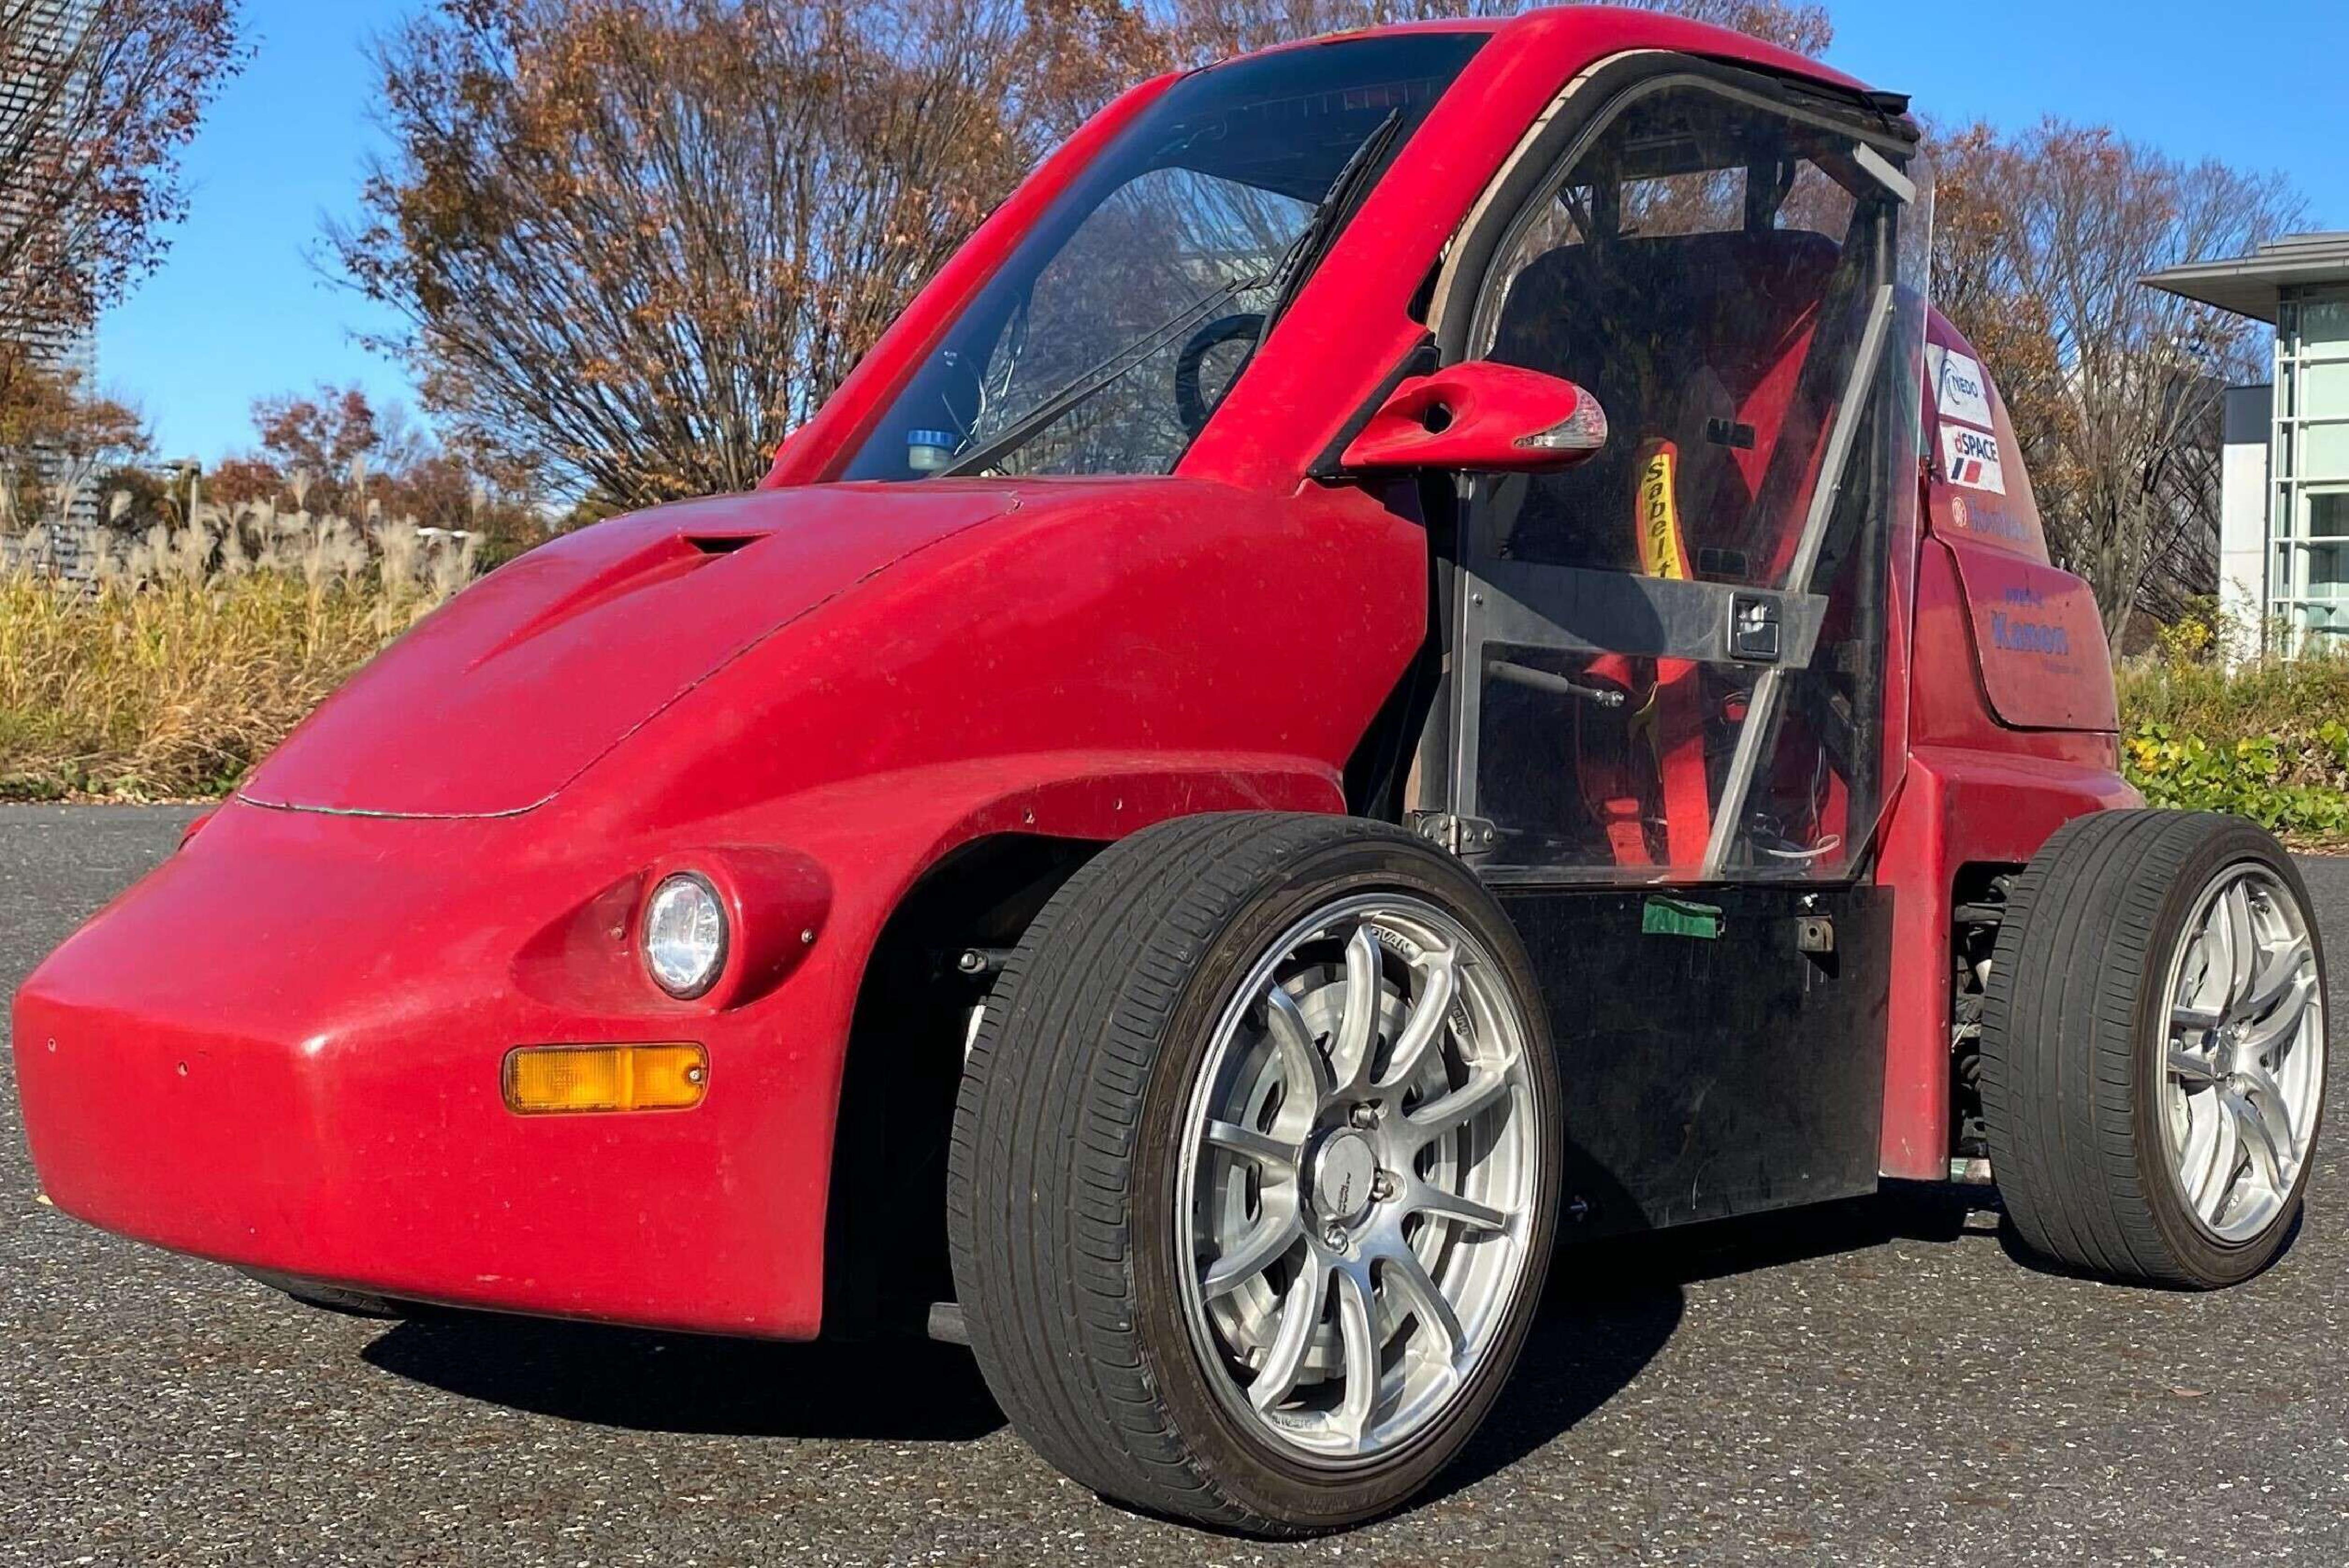
\includegraphics[width=0.45\linewidth]{fig/2_Kanon.pdf}
    \caption{FPEV-2 Kanon.}
    \label{fig:2_Kanon}
\end{figure}

\begin{table}[tb]
    \centering
    \caption{FPEV-2 Kanonの主要パラメータ.}
    \label{table:2_Kanon}
    \begin{tabular}{c c c}
        \toprule
        Symbol & Description & Value \\
        \midrule
        $M$   & Vehicle weight                  & $850\ \mathrm{kg}$ \\
        $r$   & Tire radius                    & $0.302\ \mathrm{m}$ \\
        $J_\omega$ & Wheel inertia                  & $1.24\ \mathrm{kg\,m^2}$ \\
        $T_s$ & Sampling period                & $1\ \mathrm{ms}$ \\
        $l_f$ & Distance from CG to front axle & $0.988\ \mathrm{m}$ \\
        $l_r$ & Distance from CG to rear axle  & $0.712\ \mathrm{m}$ \\
        $h_g$ & Height of center of gravity    & $0.46\ \mathrm{m}$ \\
        \bottomrule
    \end{tabular}
\end{table}

\begin{figure}[tb]

    \centering

    \begin{minipage}{0.35\linewidth}
        \centering
        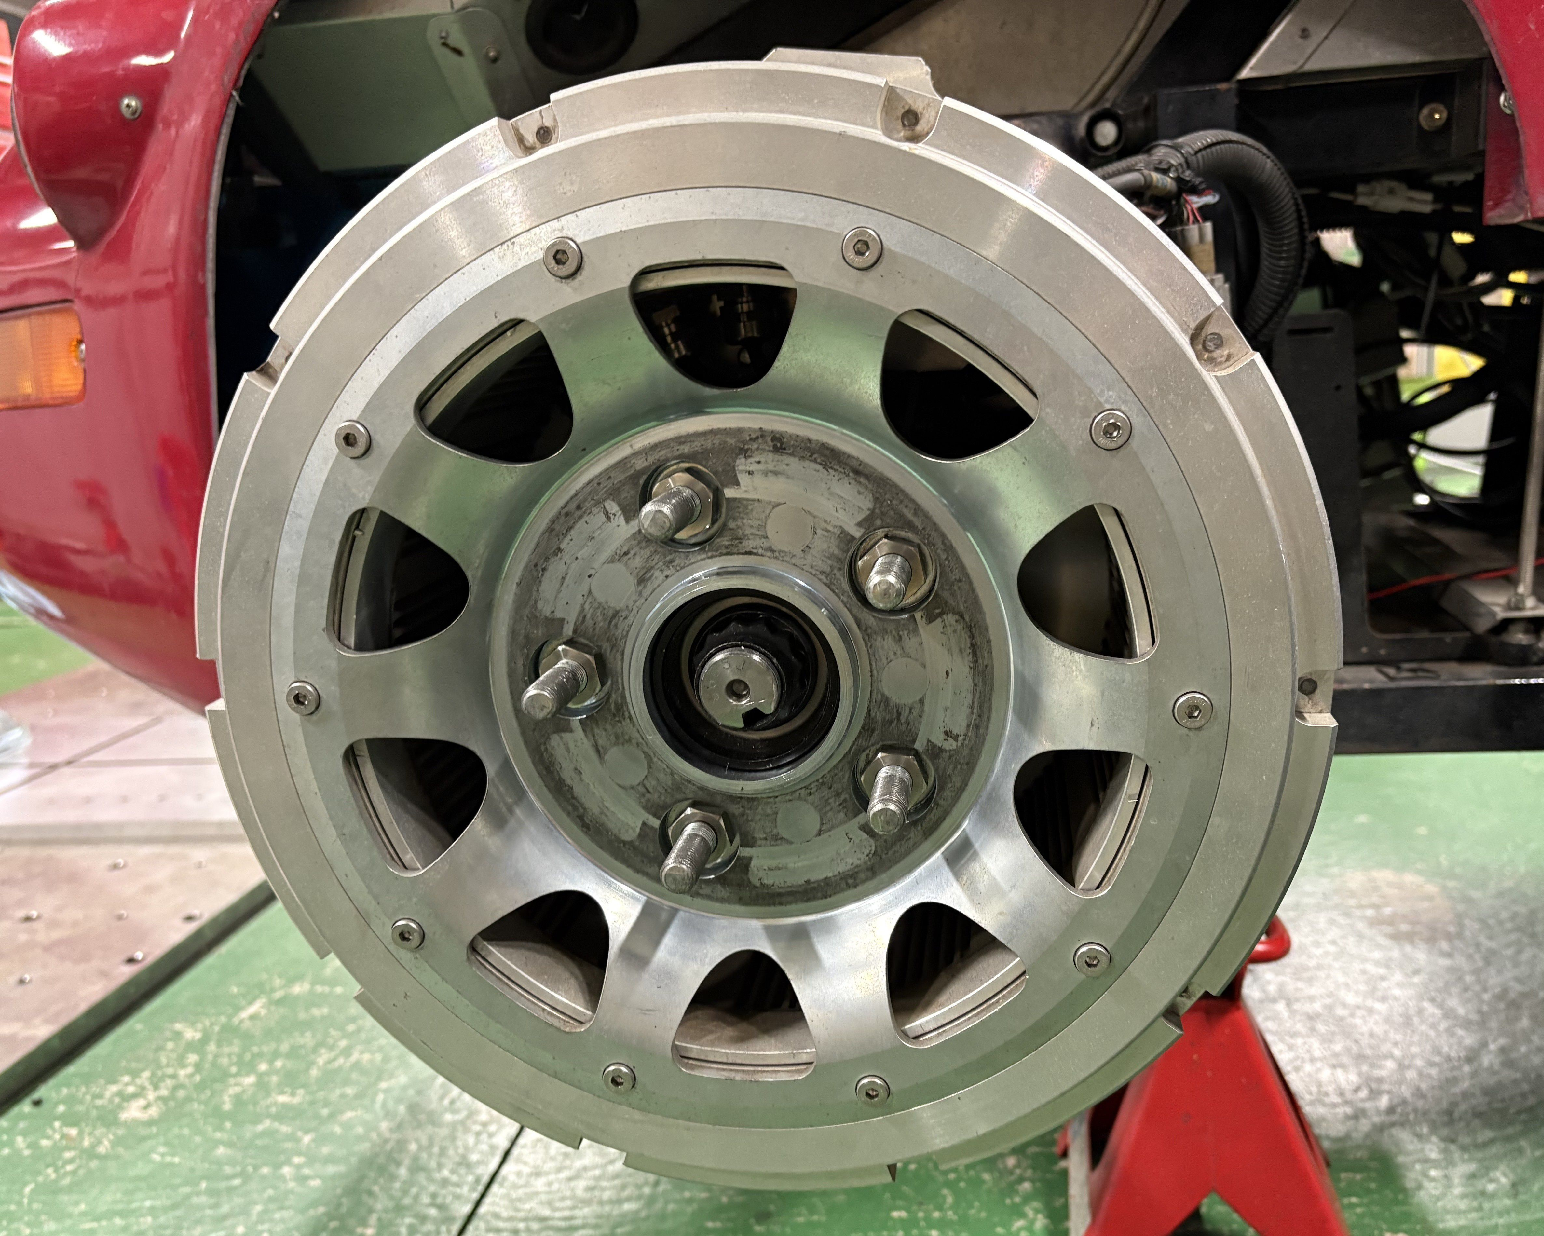
\includegraphics[
            width=\linewidth,
            height=5cm,
            keepaspectratio,
            trim=0 20 0 20,
            clip
        ]{fig/2_Kanon_front_IWM.pdf}
        \subcaption{前輪のIWM.}
        \label{fig:2_Kanon_front_IWM}
    \end{minipage}
    \hfill
    \begin{minipage}{0.35\linewidth}
        \centering
        \includegraphics[
            width=\linewidth,
            height=5cm,
            keepaspectratio,
            trim=860 20 860 20,
            clip
        ]{fig/2_Kanon_rear_IWM.pdf}
        \subcaption{後輪のIWM.}
        \label{fig:2_Kanon_rear_IWM}
    \end{minipage}

    \caption{FPEV-2 Kanonに取り付けられているインホイールモータ(IWM).}
    \label{fig:2_Kanon_IWM}

\end{figure}

\begin{table}[tb]
    \centering
    \caption{インホイールモータ(IWM)の諸元}
    \label{table:2_Kanon_IWM}
    \begin{tabular}{l c}
        \toprule
        項目 & 諸元 \\
        \midrule
        製造元       & 東洋電機製造株式会社 \\
        駆動方式     & ダイレクトドライブ \\
        定格トルク   & $110\ \mathrm{Nm}$ \\
        最大トルク   & $500\ \mathrm{Nm}$ \\
        定格出力     & $6.00\ \mathrm{kW}$ \\
        最大出力     & $20.0\ \mathrm{kW}$ \\
        定格回転速度 & $300\ \mathrm{rpm}$ \\
        最大回転速度 & $1110\ \mathrm{rpm}$ \\
        電機子抵抗   & $0.086\ \Omega$ \\
        渦電流損抵抗     & $30\ \Omega$ \\
        ヒステリシス損失 & $0.13\ \Omega$ \\
        鎖交磁束     & $0.18\ \mathrm{Wb}$ \\
        極対数       & $10$ \\
        d軸インダクタンス & $0.63\ \mathrm{mH}$ \\
        q軸インダクタンス & $0.69\ \mathrm{mH}$ \\
        \bottomrule
    \end{tabular}
\end{table}

\subsection{車両モデリング}
各車輪の回転運動の運動方程式, 以下のように表される. 
\begin{equation}
\label{eq:2_rotate_eq}
J_{\omega,ij} \dot{\omega}_{ij} = T_{ij} - rF_{\mathrm{d},{ij}}
\end{equation}

ここで, $J_{\omega,ij}$は車輪の慣性モーメント, ${\omega}_{ij}$は車輪角速度, $T_{ij}$はモータトルク, $r$は車輪半径, $F_{\mathrm{d},{ij}}$は, タイヤ・路面間に発生する路面反力, すなわち進行方向の駆動力を示す. 
なお, 添字の$i,j$は, それぞれ車輪の前後(front/rear), 車輪の左右(left/right)を示す. 
また, 車両全体の前後方向の運動方程式は以下の式で表される. 
\begin{equation}
\label{eq:2_x_eq}
M\dot{V}_x = \sum{F_{\mathrm{d},{ij}}}
\end{equation}


各タイヤの駆動力$F_{\mathrm{d},ij}$は, タイヤ-路面間の摩擦係数$\mu$と垂直荷重$F_{z,ij}$を用いて以下のように表される.
\begin{equation}
\label{eq:1_Fd}
F_{\mathrm{d},ij} = \mu F_{z,ij}
\end{equation}
また, タイヤのスリップ率$\lambda_{ij}$は以下の式で与えられる.
\begin{equation}
\label{eq:1_lambda}
\lambda_{ij} = \frac{V_{\omega,ij} - V}{\max{(V_{\omega,ij}, V, \epsilon)}}
\end{equation}
ここで, $V$は車体速度, $V_{\omega,ij}$は車輪速度であり, これは車輪角速度$\omega_{ij}$とタイヤ半径$r$から以下で表される.
\begin{equation}
\label{eq:1_V_omega}
V_{\omega,ij} = r \omega_{ij}
\end{equation}
また, $\epsilon$はゼロ割防止の微小定数である.

車両モデルは4輪モデルであり, 前後加速度に基づく荷重変動も考慮している. 前後輪の荷重は以下の式で表される.
\begin{equation}
    \label{eq:2_load_trans}
    \begin{aligned}
        F_{z,f}
        &=
        \frac{l_r}{2(l_r+l_f)}Mg
        -
        \frac{Ma_x}{2(l_r+l_f)}h_g \\
        F_{z,r}
        &=
        \frac{l_f}{2(l_r+l_f)}Mg
        +
        \frac{Ma_x}{2(l_r+l_f)}h_g
    \end{aligned}
\end{equation}
ここで, $F_{z,f}$は前輪1輪あたりの荷重, $F_{z,r}$は後輪1輪あたりの荷重, $h_g$は静止時の重心高, $l_f, l_r$はそれぞれ重心(CG)から前車軸および後車軸までの距離を表す. 
\subsection{タイヤ($\mu-\lambda$特性)モデリング}
前述の通り, $\mu-\lambda$曲線は路面やタイヤ状態により異なり, 形状も非線形性を持つ.
これに対し, Pacejkaらにより経験的なデータからフィッティングされた, Magic Formula\cite{pacejka}というタイヤモデルが存在する. 
Magic Formulaを以下の式に示す. 
\begin{equation}
    \label{eq:2_magicformula}
    \mu_{ij}
    =
    D\sin\left(
    C\arctan(B\lambda_{ij})
    -
    E\left(
    B\lambda_{ij}
    -
    \arctan(B\lambda_{ij})
    \right)
    \right)
    \end{equation}
ここで, $B$はStiffness factor, $C$はShape factor, $D$はPeak factor, $E$はCurvature factorと呼ばれる係数であり, この4つの係数により, $\mu-\lambda$曲線をフィッティングしている. 
これらは直接的な物理パラメータではなく,実験データへのフィッティングによって決定される経験的な係数である.
このモデルはタイヤの非線形特性などを高精度に表現できるため, 多くの研究において標準的なタイヤモデルとして広く用いられている.

\subsection{実験機器:インタイヤハウスダイナモ(ITHD)}
実験機器として用いた, 東洋電機製造株式会社製の台上試験機「インタイヤハウスダイナモ(In-Tire-House Dynamo : ITHD)」\cite{ithd}について述べる. 
従来のシャシダイナモメータは円筒状のローラを用いて車両の走行を模擬していたが, ITHDはハブダイナモの一種であり, ダイナモメータをIWMに直接接続しダイナモメータにより車輪に作用する負荷トルクを直接模擬する.
この構造により, 系を低慣性にし, 高精度な周波数応答の再現・計測が可能となる.
また, 屋内の試験設備であることから試験場の広さに依存せず, 走行試験に相当する条件で実験を行うことができる他, 路面モデルを指定することで試験場では再現が困難な様々な路面上における走行を再現できる.
本研究で使用したITHDの主要な諸元をTable \ref{table:2_ITHD}に示す. 

\begin{table}[tb]
    \centering
    \caption{ITHDの主要諸元}
    \label{table:2_ITHD}
    \begin{tabular}{lc}
        \hline
        項目 & 数値 \\
        \hline
        定格容量 & 94.2 kW \\
        最大回転数 & 2,000 min$^{-1}$ \\
        最大瞬間トルク & 1,350 Nm \\
        装置外形（直径） & 650 mm \\
        トレッド幅（ダイナモ本体） & 185 mm \\
        最大対応ブレーキ（直径） & 425 mm \\
        \hline
    \end{tabular}
\end{table}

%%========== 第3章 ==========%%
\clearpage
\section{駆動力制御 (DFC)}
\subsection{スリップ率制御}
DFCは, 前述の通りカスケード構造をしているが, 駆動力指令値$F^*_\mathrm{d}$に対しI制御を行うことでまずスリップ率指令値に変換しており, それ以降でスリップ率制御を行っている.
一方, スリップ率$\lambda$は式(\ref{eq:1_lambda})に示す通り, 駆動時($V_\omega \ge V$)と制動時($V_\omega < V$)で定義が異なるため, 制御上で不都合が生じる. 
そのため, スリップ率$\lambda$の代わりに, 操作量$y$を用いて制御を行う. $y$を以下の式に示す. 
\begin{equation}
\label{eq:3_y}
y_{ij} = \frac{V_{\omega,ij} - V}{V} = \frac{V_{\omega,ij}}{V} - 1
\end{equation}
また, スリップ率$\lambda$との関係は以下の式で表される. 
\begin{equation}
    \label{eq:3_y_lambda}
    y_{ij}
    =
    \begin{cases}
    \frac{\lambda}{1 - \lambda} & (V_{\omega,ij} \ge V) \\
    \lambda & (V_{\omega,ij} < V)
    \end{cases}
\end{equation}

この$y$を用いて, 車輪速制御の指令値$V_{\omega}^{*}$は以下のように表すことができる. 
\begin{equation}
    \label{eq:3_V_omega}
    V_{\omega}^{*} = V(1+y) 
\end{equation}
車輪速制御はPI制御であり, この出力がIWMへのトルク指令値$T^*$となる. 

\subsection{駆動力オブザーバ(Driving Force Observer : DFO)}
駆動力制御では, 駆動力オブザーバ(Driving Force Observer : DFO)\cite{hori}により出力された駆動力を推定し, フィードバック制御を行う. 
DFOでは, 前述の回転方向運動方程式(式(\ref{eq:2_rotate_eq}))を変形することで, 駆動力を推定している. 
ブロック線図をFig.\ref{fig:3_DFO}に示す. 
\begin{figure}[tb]
    \centering
    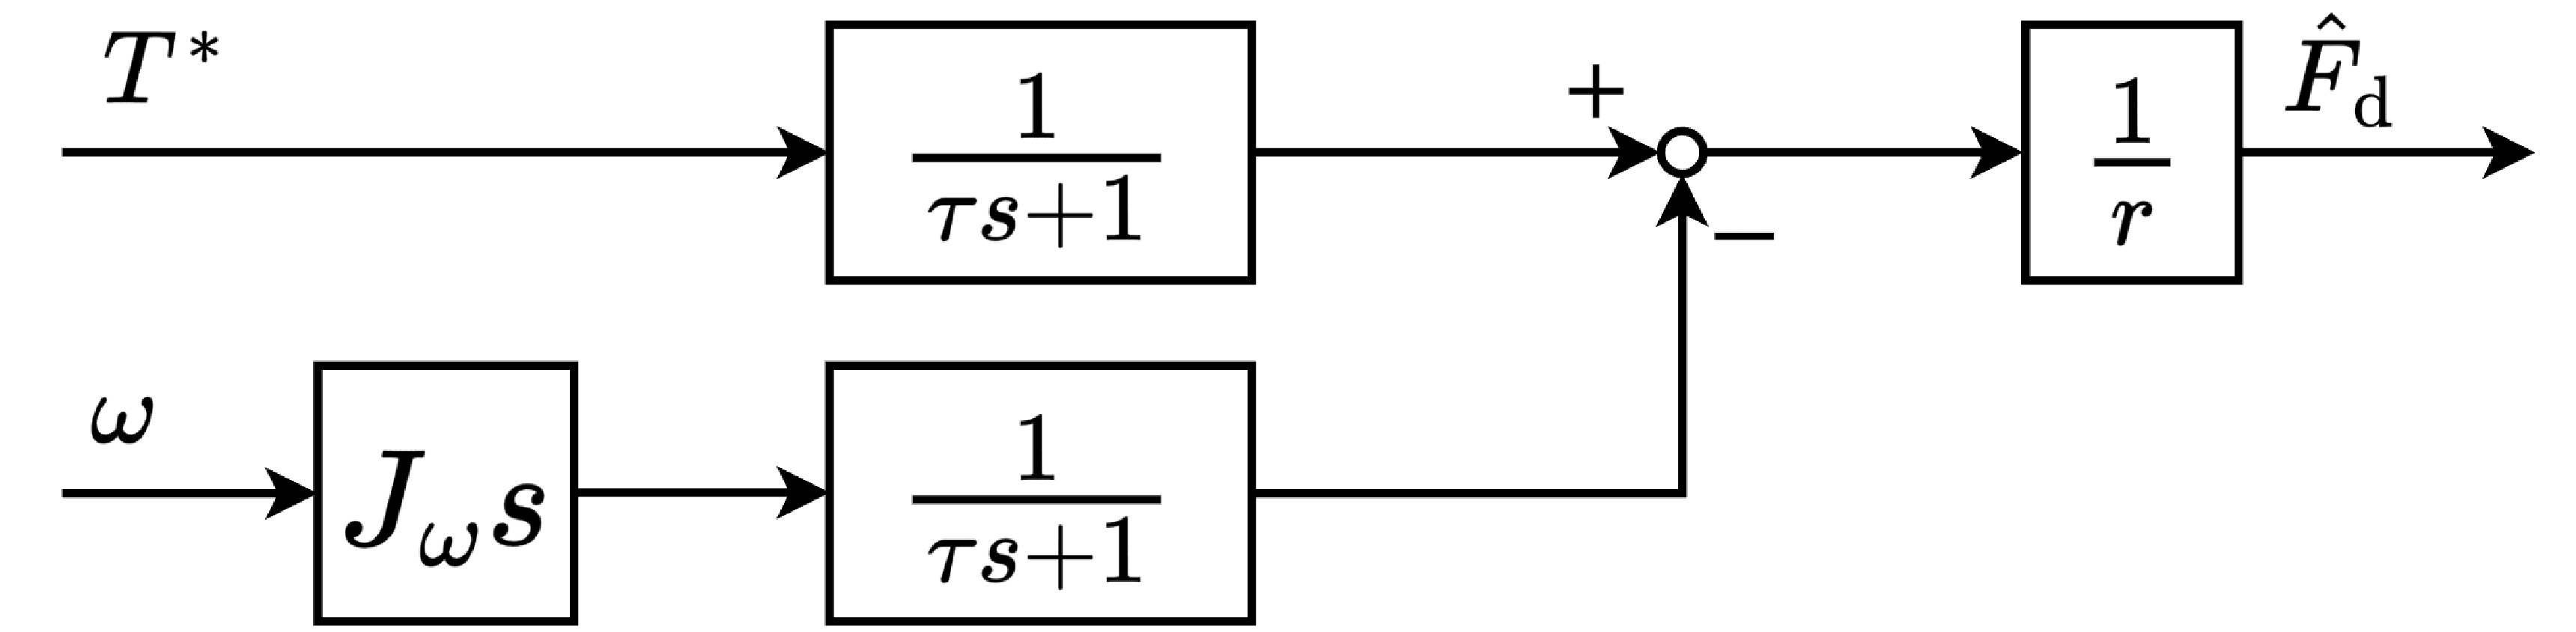
\includegraphics[width=0.8\linewidth]{fig/3_DFO.pdf}
    \caption{DFOのブロック線図.}
    \label{fig:3_DFO}
\end{figure}
また, 推定される駆動力の数式を以下に示す. 
\begin{equation}
\label{eq:3_DFO}
\hat{F}_{\mathrm{d},{ij}} = Q_f(s) \frac{T^*_{ij} - J_{\omega,ij}{\dot{\omega}}_{ij}}{r}
\end{equation}
ここで用いている$Q_f(s) = 1 / (\tau_f s + 1)$は時定数$\tau_f$の一次のローパスフィルタである. 
また,${\dot{\omega}}_{ij}$は, 車両に取り付けられたエンコーダから読み取った車輪角速度${\omega}_{ij}$を擬似微分することにより求められる.

%%============== 第4章 ============%%
\clearpage
\section{機械学習を用いた$\mu-\lambda$曲線推定を伴う$\lambda_{\mathrm{peak}}$推定}
\subsection{手法概要}
本研究の提案手法では, 観測された点$(\hat{\mu},\hat{\lambda})$の情報から, はじめに$\mu-\lambda$曲線の形状を推定し, 推定された曲線からピーク点を判定するという流れを踏んでいる. 
$\mu-\lambda$曲線推定のフローチャートをFig.\ref{fig:4_prop_flow}に示す.
実際の走行時には, 十分に広い範囲の$\lambda$の情報を得ることができない. そのため機械学習を用いて, 観測できていない範囲の$\mu-\lambda$曲線を推定する. 
機械学習モデルは, ニューラルネットワークの一種である多層パーセプトロン(Multi Layer Perceptron : MLP)を用い, オフラインで学習を行った後実測された摩擦係数およびスリップ率の情報から$\mu-\lambda$曲線を推定する.

\begin{figure}[tb]
    \centering
    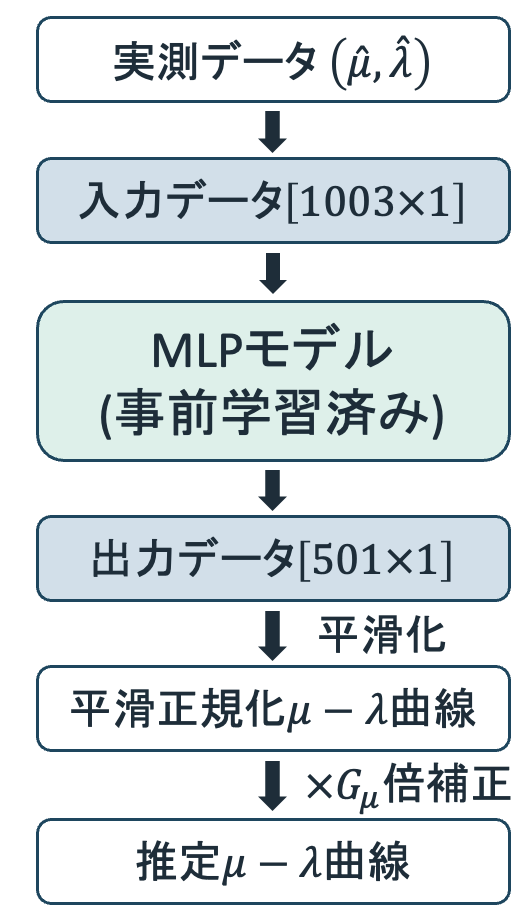
\includegraphics[width=0.25\linewidth]{fig/4_prop_flow.png}
    \caption{提案手法のフローチャート.}
    \label{fig:4_prop_flow}
\end{figure}

推定された$\mu-\lambda$曲線から最適スリップ率$\hat{\lambda}_\mathrm{peak}$を推定し, この数値をスリップ率リミッタに適用$(\lambda_\mathrm{lim} = \hat{\lambda}_\mathrm{peak})$することで, 駆動力制御中の走行安定性向上と駆動力最大化を両立する. 

\subsection{$\mu-\lambda$曲線}
\subsubsection{実測データ}
推定に使う測定データは, 逐次EVから得られる摩擦係数の推定値$\hat{\mu}$とスリップ率の推定値$\hat{\lambda}$である. 
$\hat{\mu}$については, 以下の式で表される.

\begin{equation}
\label{eq:4_mu_hat}
\hat{\mu}_{ij} = \frac{\hat{F}_{\mathrm{d},{ij}}}{\hat{F}_{z,i}}
\end{equation}
ここで, $\hat{F}_\mathrm{d}$は式(\ref{eq:3_DFO})で示される駆動力推定値$\hat{F}_\mathrm{d}$であり, $\hat{F}_{z,i}$は各車輪の垂直荷重の推定値である. 
具体的には, 式(\ref{eq:2_load_trans})をもとに, 
\begin{equation}
    \label{eq:4_load_trans_hat}
    \begin{aligned}
        \hat{F}_{z,f}
        &=
        \frac{l_r}{2(l_r+l_f)}Mg
        -
        \frac{M{a}_x}{2(l_r+l_f)}h_g \\
        \hat{F}_{z,r}
        &=
        \frac{l_f}{2(l_r+l_f)}Mg
        +
        \frac{M{a}_x}{2(l_r+l_f)}h_g
    \end{aligned}
\end{equation}
と表される. ${a}_x$は車両の前後方向の加速度推定値であり, これはIMU(慣性計測ユニット)により計測される値である.

また, スリップ率推定値$\hat{\lambda}$は以下の式で表される. 
\begin{equation}
\label{eq:4_lambda_hat}
\hat{\lambda}_{ij} = \frac{V_{\omega,ij} - V}{\max{(V_{\omega,ij}, V, \epsilon)}} = \frac{r{\omega}_{ij} - V}{\max{(r{\omega}_{ij}, V, \epsilon)}} 
\end{equation}
${\omega}_{ij}$は駆動輪の車輪角速度であり, インホイールモータに取り付けられたエンコーダから測定される.
また, 今回は前輪2輪駆動を考えているため, 後輪は従動輪となっている. この時, 車体速度${V}$は, 車輪半径$r$と従動輪の車輪角速度との積で求められる. 

\subsubsection{入力データ}
機械学習(MLP)モデルに実測値を入力する際には, 測定された点をそのまま入力するのではなく, 一定の加工を行うことによって$\lambda$分布が部分的な状態から$\mu-\lambda$曲線全体を復元できるようにする.
概要を表す図をFig.\ref{fig:4_2_input}に示す. 

\begin{figure}[tb]
    \centering

    \begin{minipage}{0.45\linewidth}
        \centering
        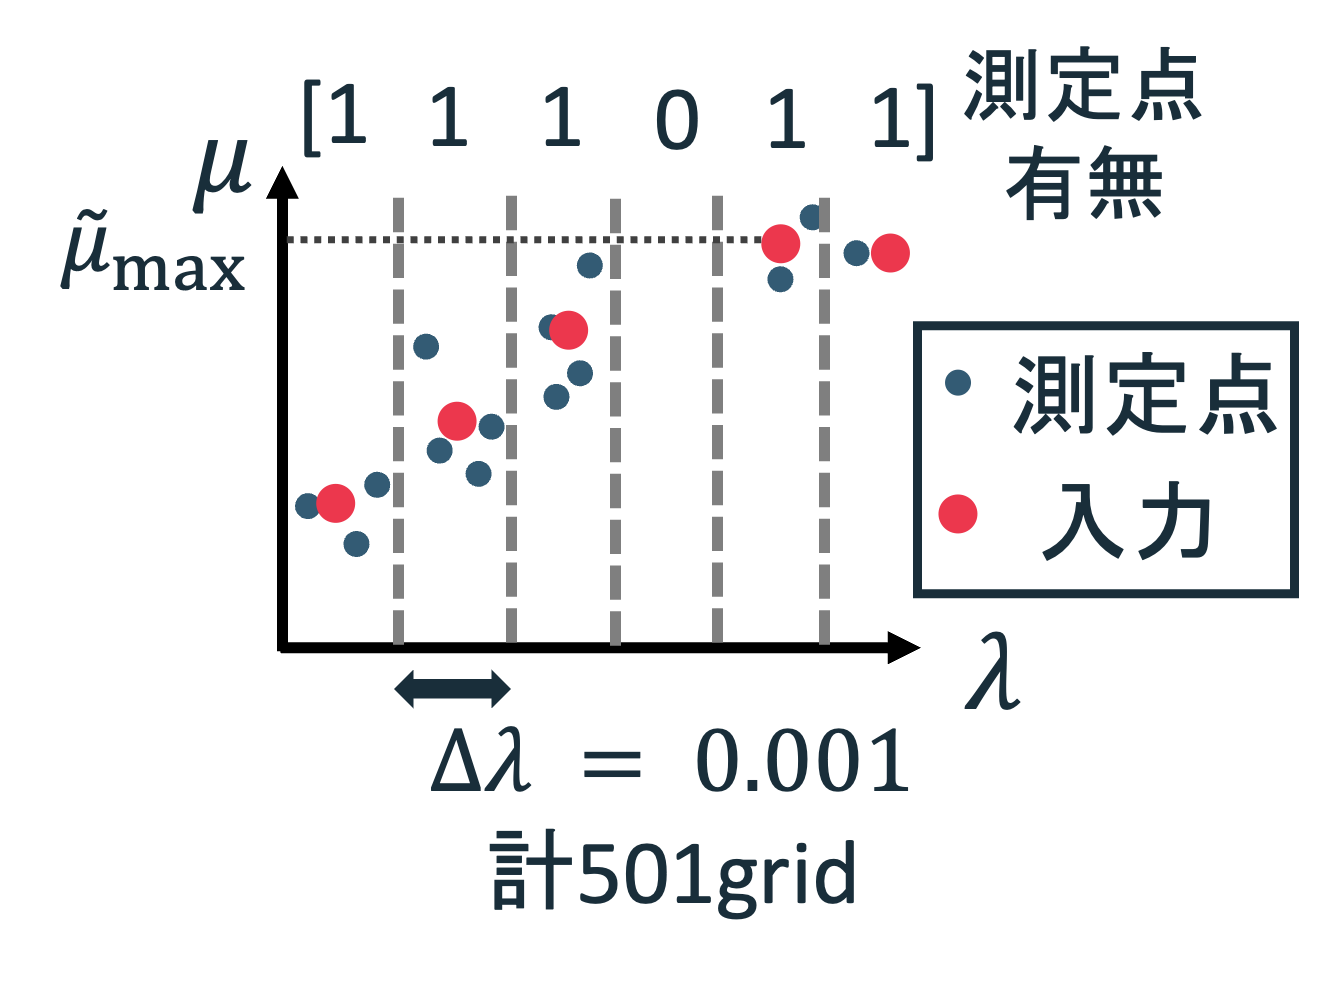
\includegraphics[height=45mm]{fig/4_2_input.png}
        \captionof{figure}{MLP入力のイメージ図.}
        \label{fig:4_2_input}
    \end{minipage}
    \hfill
    \begin{minipage}{0.45\linewidth}
        \centering
        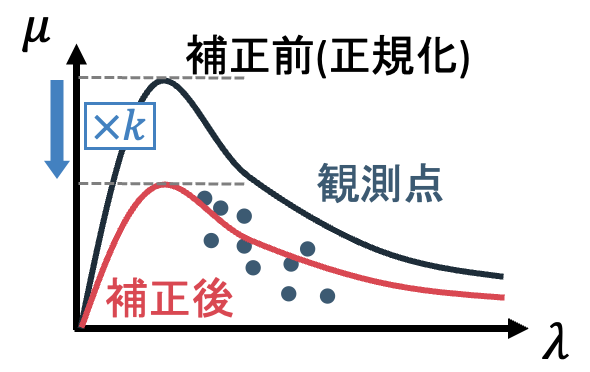
\includegraphics[height=45mm]{fig/4_2_output.png}
        \captionof{figure}{スケール補正のイメージ図.}
        \label{fig:4_2_output}
    \end{minipage}
\end{figure}

まず, 実測した$\mu-\lambda$プロットを, $0 \le \lambda \le 0.5$の範囲で, 幅$\Delta \lambda = 0.001$の計501グリッドに分類する. 
その後, 各グリッド内の点の$\mu$の平均値をそのグリッドの代表値として用い, $0 \le \lambda \le 0.5$の範囲で$\mu-\lambda$曲線を計501点の離散化曲線とする. 
この曲線部分は$[501\times1]$のベクトル$\bm{\mu}_{\mathrm{in},k}$と表すことができる. 
この時, グリッド内に測定点が含まれない場合は, 0として扱う. 

次に, 部分的な観測情報から曲線全体を復元するための情報として, どのグリッドにおいて測定点が存在するかを入力する. 
測定点が存在するグリッドに対しては1, 存在しないグリッドは0とし, こちらも$[501\times1]$のベクトル$\bm{m}_{k}$と表すことができる. 

また, 詳しくは学習方法のセクションにおいて後述するが, 観測されている中の$\mu$最大値($=\tilde{\mu}_\mathrm{max}$)で正規化を行う. 
正規化された入力を$\bm{\mu}_{\mathrm{in,norm},k}$とする.

この時入力データは$\mu$スケールの情報を持たなくなるが, 曲線復元の情報としてMLPモデルに$\tilde{\mu}_\mathrm{max}$も入力する.

したがって, MLPへの入力は,
正規化された観測$\mu$の501点(=$\bm{\mu}_{\mathrm{in,norm},k}$), 観測マスクの501点(=$\bm{m}_{k}$),
および観測$\mu$最大値$\tilde{\mu}_{\mathrm{max}}$の1点から構成され,
合計$501+501+1=1003$次元となる.

\subsubsection{出力データ}
MLPモデルの出力は, 入力と同様に501点の離散化曲線として, $[501\times1]$サイズのベクトル$\bm{\mu}_{\mathrm{out,norm},k}$となる. 
一方, 生の出力データは離散化されかつ正規化された状態であり, 出力点自体も細かく上下に振動しているため, このままでは実際の$\mu-\lambda$とは異なる状態であり加工が必要である. 
そこで, まずはじめに出力の平滑化を行い, 連続かつ滑らかな曲線にする. 平滑化には, 多項式次数3, フレーム長51点のSavitzky-Golay filterを用いた. 

次に, 正規化曲線を, 実測スケールに戻す手順を行う. イメージ図をFig.\ref{fig:4_2_output}に示す.
具体的には, スケール補正後の曲線と観測点とのRMSEが最小になるように, スケール補正前の正規化曲線にゲイン$G_\mu$をかける. 
$G_\mu$は以下の式で計算される.
\begin{equation}
    G_{\mu,k}
    =
    \frac{
    \displaystyle \sum_{m_{k,i}=1}
    \mu_{\mathrm{out,norm},{k,i}}\mu_{\mathrm{in},{k,i}}
    }{
    \displaystyle \sum_{m_{k,i}=1}
    \mu_{\mathrm{out,norm},{k,i}}^{2}
    }
\end{equation}
ここで, $G_{\mu,k}$は時刻(ステップ)$k$におけるゲインであり, $\mu_{\mathrm{in},{k,i}}$は時刻$k$における入力の$i$番目のグリッドの値, $\mu_{\mathrm{out,norm},{k,i}}$は平滑化後の正規化出力曲線を表す. 

\subsubsection{オフライン学習}
本研究では, 機械学習モデルとして多層パーセプトロン(Multi Layer Perceptron : MLP)を使用し, オフラインで学習を行う. 

学習用の教師データ・入力データはいずれもシミュレーションデータを用いて作成した. シミュレーション環境はMATLAB/Simulinkを用いた. 車両モデルは荷重変動を考慮した4輪モデルであり, タイヤモデルは前述のMagic Formulaを用いた. 
Magic Formulaのパラメータを調整することで, 様々な種類の路面パターンを再現した. 

教師データは車両プラントモデルから取得される真$\mu-\lambda$曲線とした. 
入力データは, シミュレーションにおいてスリップ率制御を用いて$0\le \lambda \le 0.5$の範囲で十分に測定点を取得したデータを用いる. 
一方, 実走行のオンライン推定時には, 観測できるデータは$0\le \lambda \le 0.5$のうち一部分しか存在していないため, 学習時にもその部分情報を再現するため, ランダムな範囲で観測範囲を制限した. 
ランダムな範囲の設定には, $0 \le  p \le 1$を満たすランダムな数値$p$を用い, $p$の値で観測範囲をランダムに設定した.
加えて, 入力点数を200点(0.2秒分の観測データ)に制限することでリアルタイムの推定を学習するように設定している. 
以上の加工により, 学習用の入力データにおいて, 実走行時のデータ点を再現した. 

MLPの損失関数には, 教師データと出力のRMSE($L_\mathrm{Data}$)と, 入力と出力のRMSE($L_\mathrm{Input}$)の2種類を設定した. 
$L_\mathrm{Data}$は一般的な機械学習モデルで使われる, 教師データを学習するための損失である.
$L_\mathrm{Input}$は入力点をそのまま出力させるような損失であり, これを用いることで, 出力曲線が学習データに依存しすぎず, 実測点に追従するような効果をもたらすことができる.
そして, 全体の損失関数を以下のように設定する. 
\begin{equation}
\label{eq:4_2_loss}
L_\mathrm{Total} = 0.1 L_\mathrm{Data} + 1.0 L_\mathrm{Input}
\end{equation}
上のように, $L_\mathrm{Input}$を$L_\mathrm{Data}$に対し10倍強く設定することで, データが観測できている領域においては実測点の形状に強く追従させることができる. 観測できていない範囲においては, $L_\mathrm{Input}$は0となることから, 教師データの形状を出力する形になり, 未観測の領域においても自然な$\mu-\lambda$曲線を補完することができる.

機械学習の学習データ$\mu-\lambda$曲線は複数パターン存在するものの, $\mu-\lambda$曲線の推定結果が学習した曲線の形状に強く影響を受ける可能性がある.
一方, 本研究の目的としてあらゆる路面に対し$\mu-\lambda$曲線を推定することを考えているため, できるだけ学習曲線の形状だけでなく未知形状の$\mu-\lambda$曲線も推定したい. 
そのため, 入力データについて, 観測されている中の$\mu$最大値($=\tilde{\mu}_\mathrm{max}$)で正規化を行う. 
これにより, 入力データは$\mu$スケールの情報を持たなくなり, 学習データの$\mu$スケールによらずに形状を復元することが可能になる. 

%%=============== 第5章 =================%%
\clearpage

\begin{figure}[tb]
    \centering
    \begin{minipage}{0.45\linewidth}
        \centering
        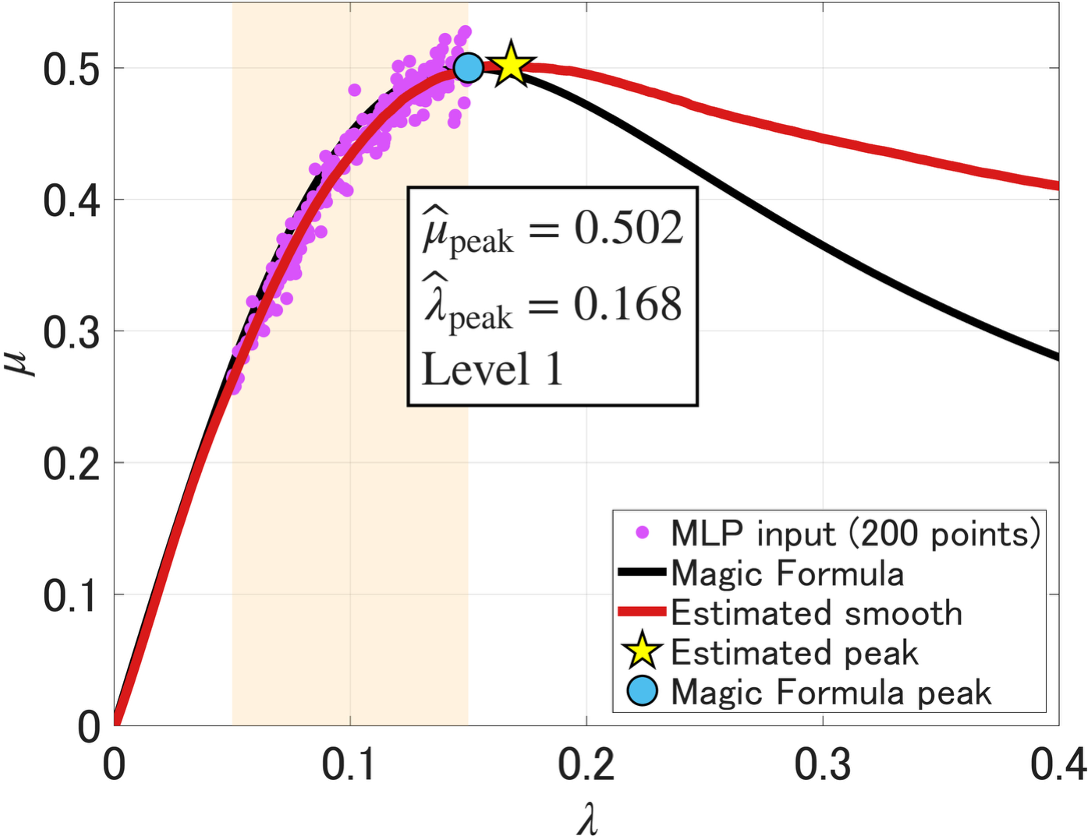
\includegraphics[width=\linewidth]{fig/5_road80_0.05_0.15_curve.png}
        \subcaption{路面1 / 観測範囲 : $0.05\le\lambda\le0.15$.}
        \label{fig:5_road80_0.05_0.15_curve}
    \end{minipage}
    \hfill
    \begin{minipage}{0.45\linewidth}
        \centering
        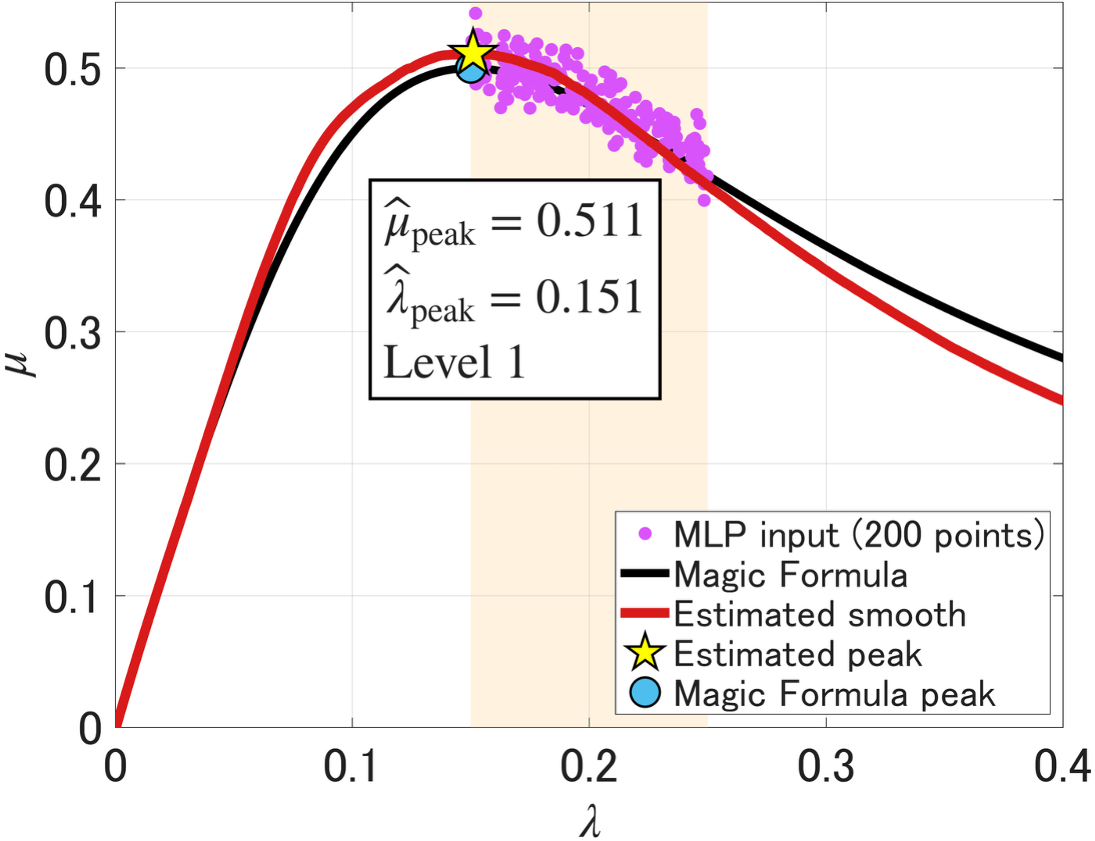
\includegraphics[width=\linewidth]{fig/5_road80_0.15_0.25_curve.png}
        \subcaption{路面1 / 観測範囲 : $0.15\le\lambda\le0.25$.}
        \label{fig:5_road80_0.15_0.25_curve}
    \end{minipage}

    \vspace{0.5em}

    \begin{minipage}{0.45\linewidth}
        \centering
        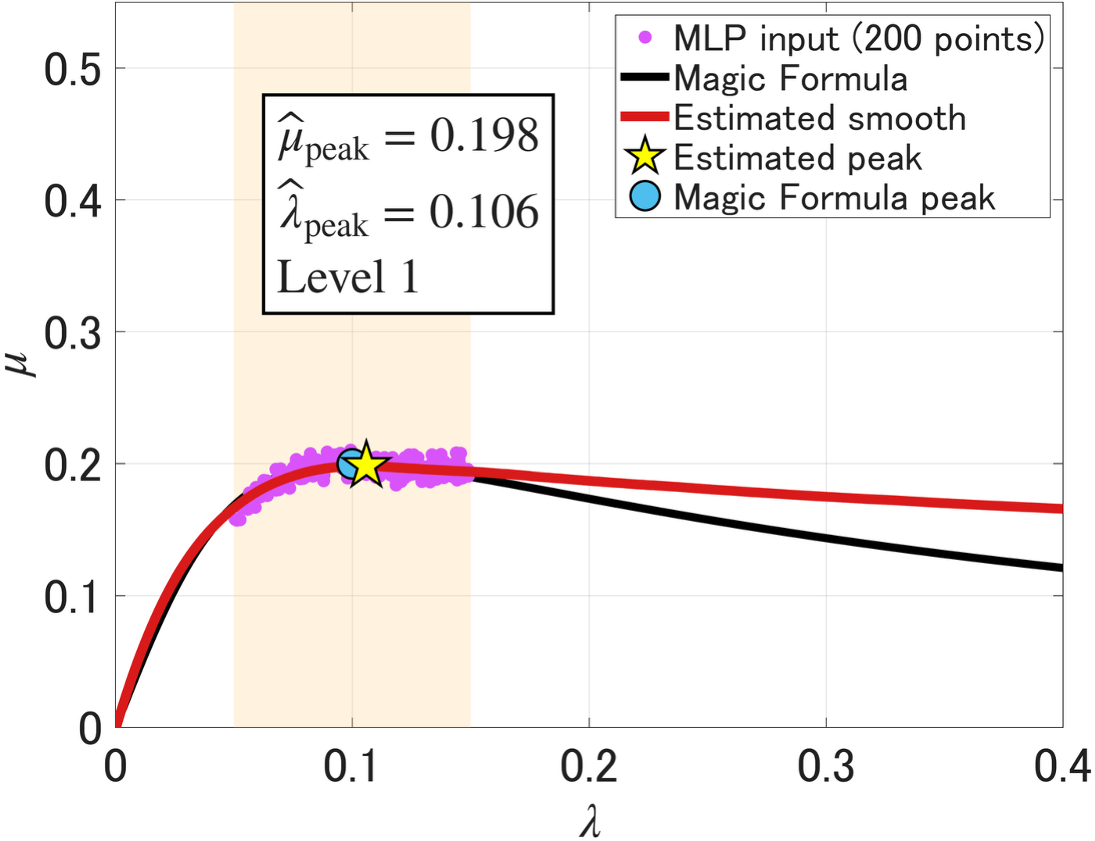
\includegraphics[width=\linewidth]{fig/5_road81_0.05_0.15_curve.png}
        \subcaption{路面2 / 観測範囲 : $0.05\le\lambda\le0.15$.}
        \label{fig:5_road81_0.05_0.15_curve}
    \end{minipage}
    \hfill
    \begin{minipage}{0.45\linewidth}
        \centering
        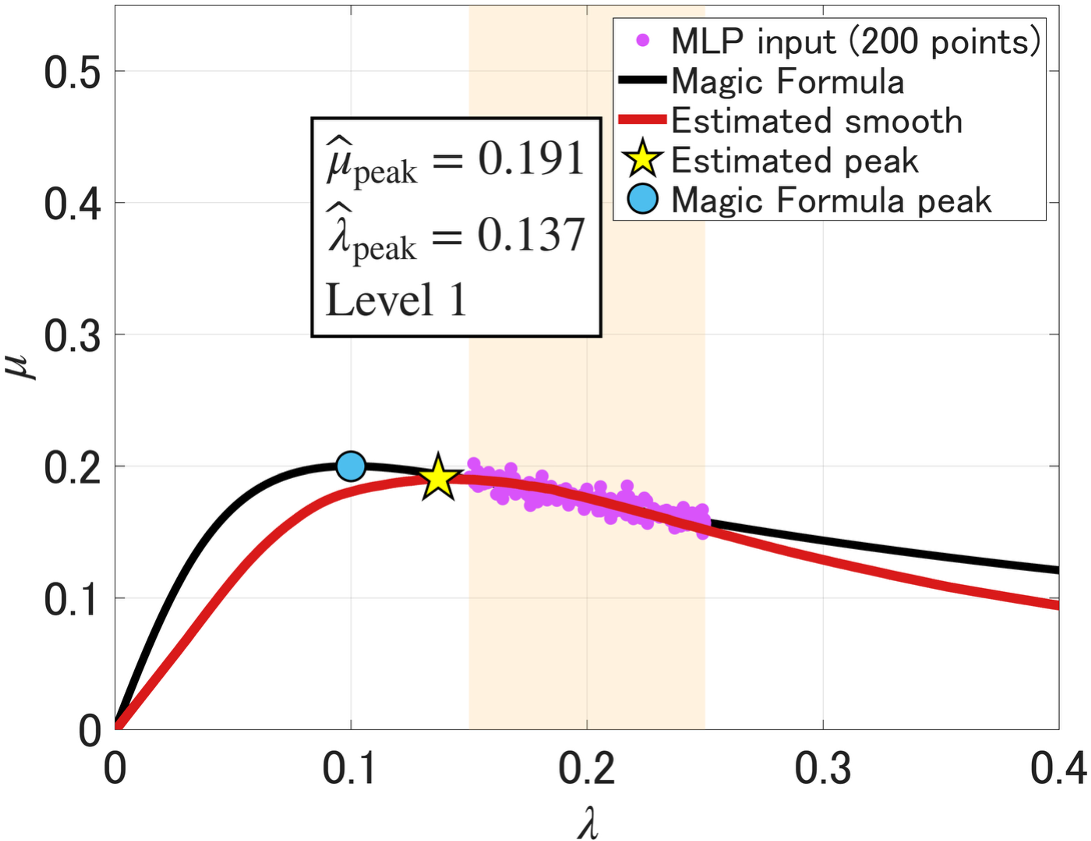
\includegraphics[width=\linewidth]{fig/5_road81_0.15_0.25_curve.png}
        \subcaption{路面2 / 観測範囲 : $0.15\le\lambda\le0.25$.}
        \label{fig:5_road81_0.15_0.25_curve}
    \end{minipage}
    \caption{部分観測情報からの曲線・ピーク点推定結果.}
    \label{fig:5_result_curve}
\end{figure}
\begin{figure}[tb]
    \centering
    \begin{minipage}{0.45\linewidth}
        \centering
        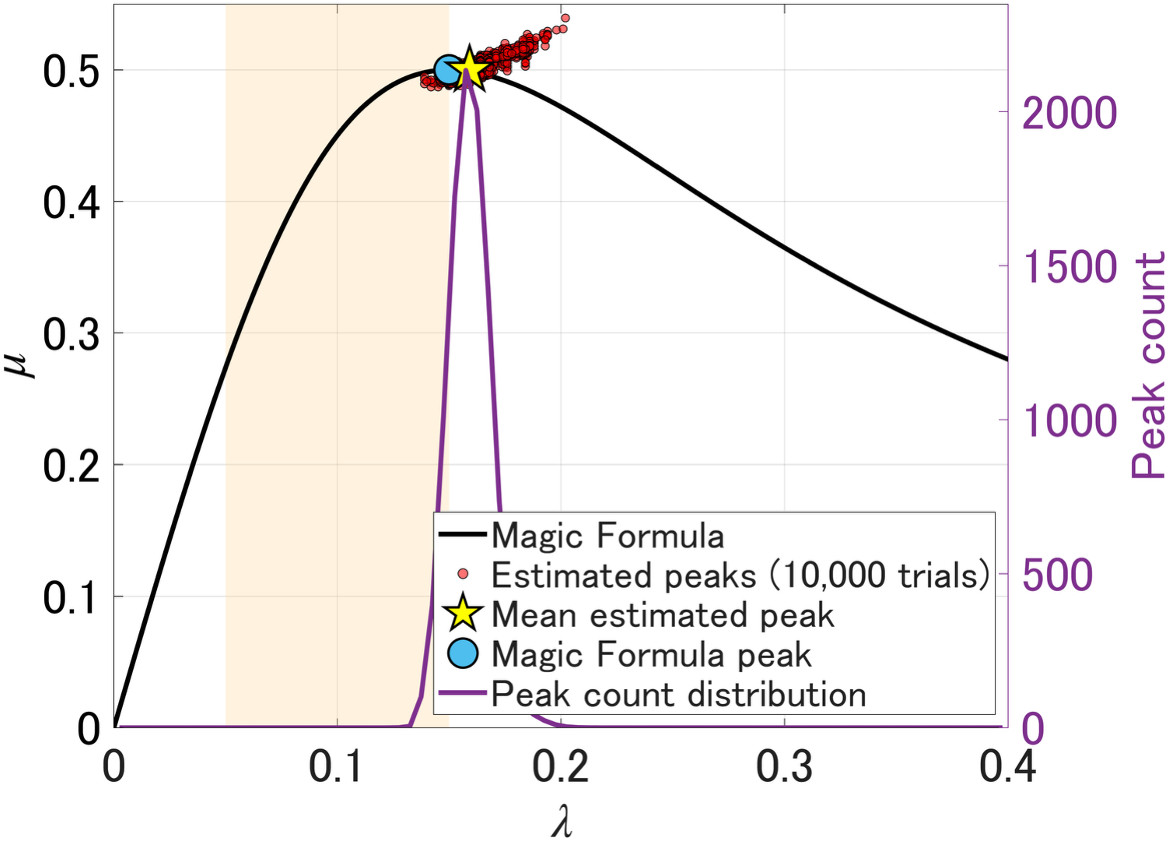
\includegraphics[width=\linewidth]{fig/5_road80_0.05_0.15_10000.png}
        \subcaption{路面1 / 観測範囲 : $0.05\le\lambda\le0.15$.}
        \label{fig:5_road80_0.05_0.15_10000}
    \end{minipage}
    \hfill
    \begin{minipage}{0.45\linewidth}
        \centering
        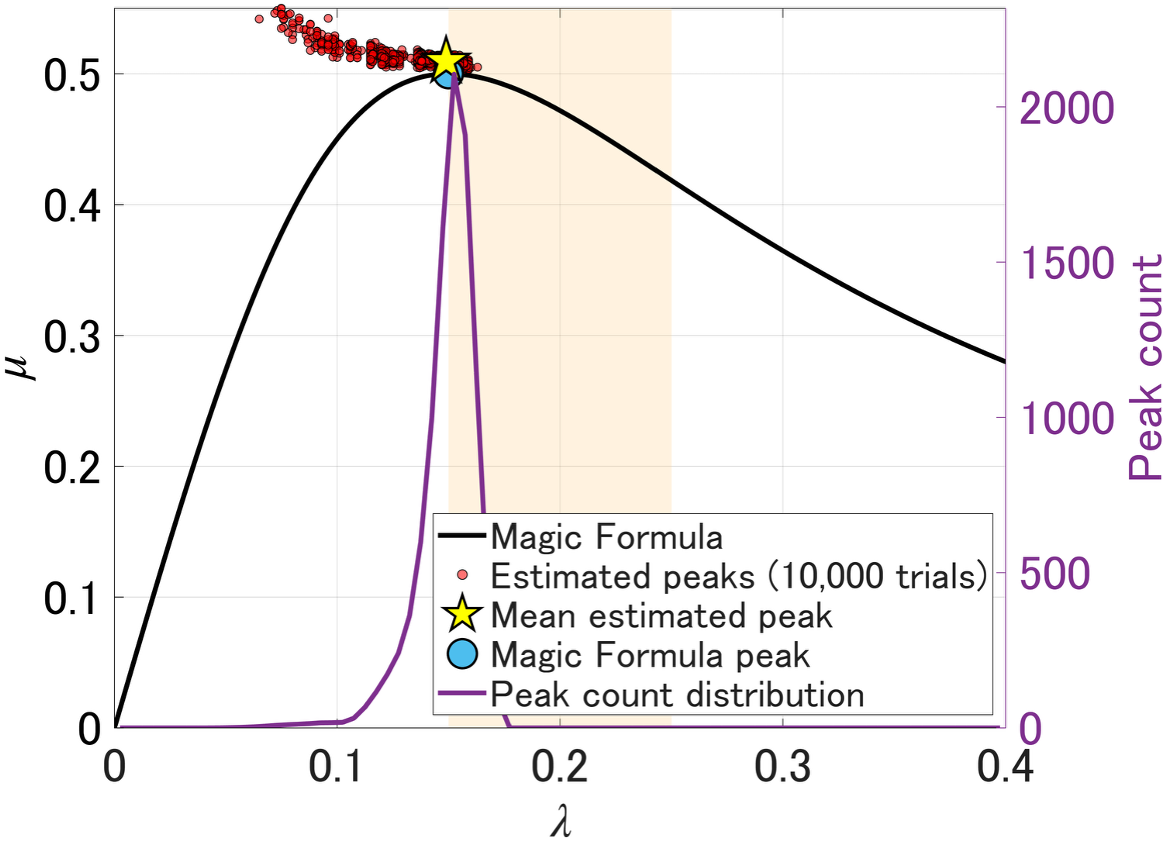
\includegraphics[width=\linewidth]{fig/5_road80_0.15_0.25_10000.png}
        \subcaption{路面1 / 観測範囲 : $0.15\le\lambda\le0.25$.}
        \label{fig:5_road80_0.15_0.25_10000}
    \end{minipage}
    \vspace{0.5em}
    \begin{minipage}{0.45\linewidth}
        \centering
        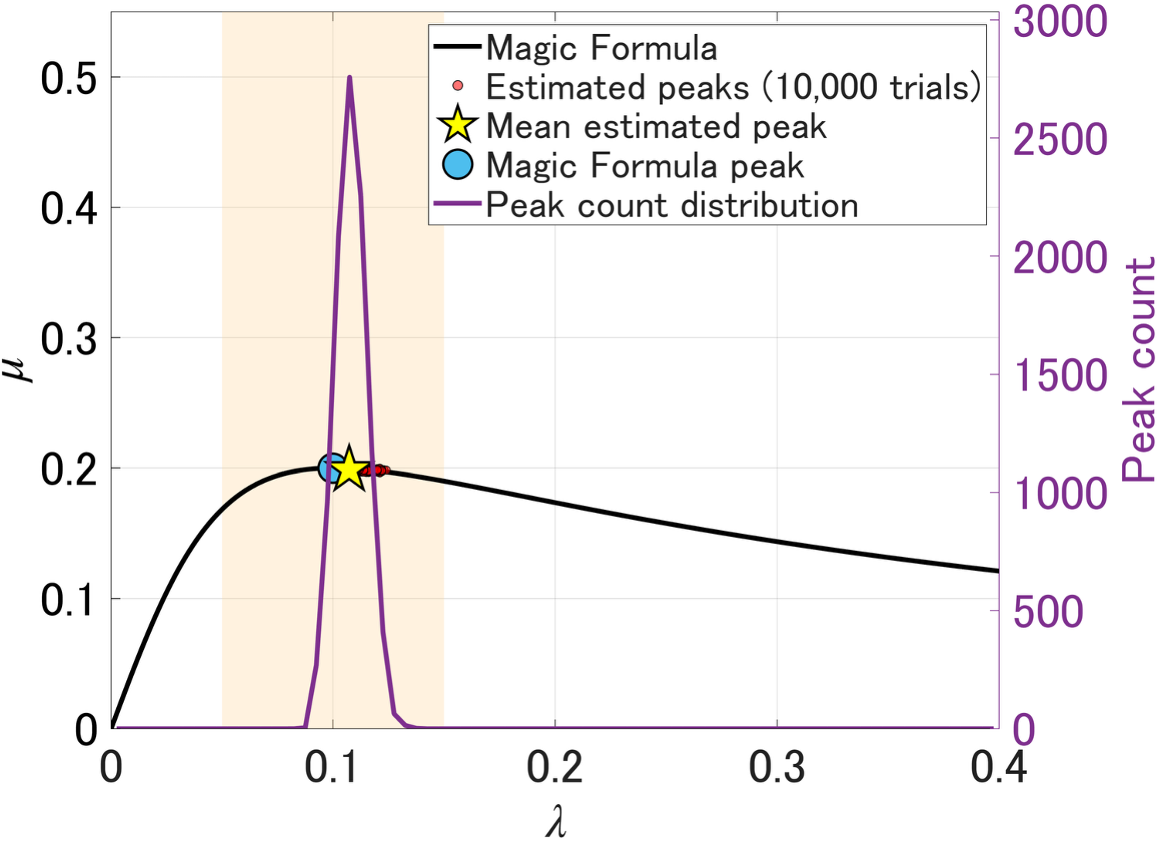
\includegraphics[width=\linewidth]{fig/5_road81_0.05_0.15_10000.png}
        \subcaption{路面2 / 観測範囲 : $0.05\le\lambda\le0.15$.}
        \label{fig:5_road81_0.05_0.15_10000}
    \end{minipage}
    \hfill
    \begin{minipage}{0.45\linewidth}
        \centering
        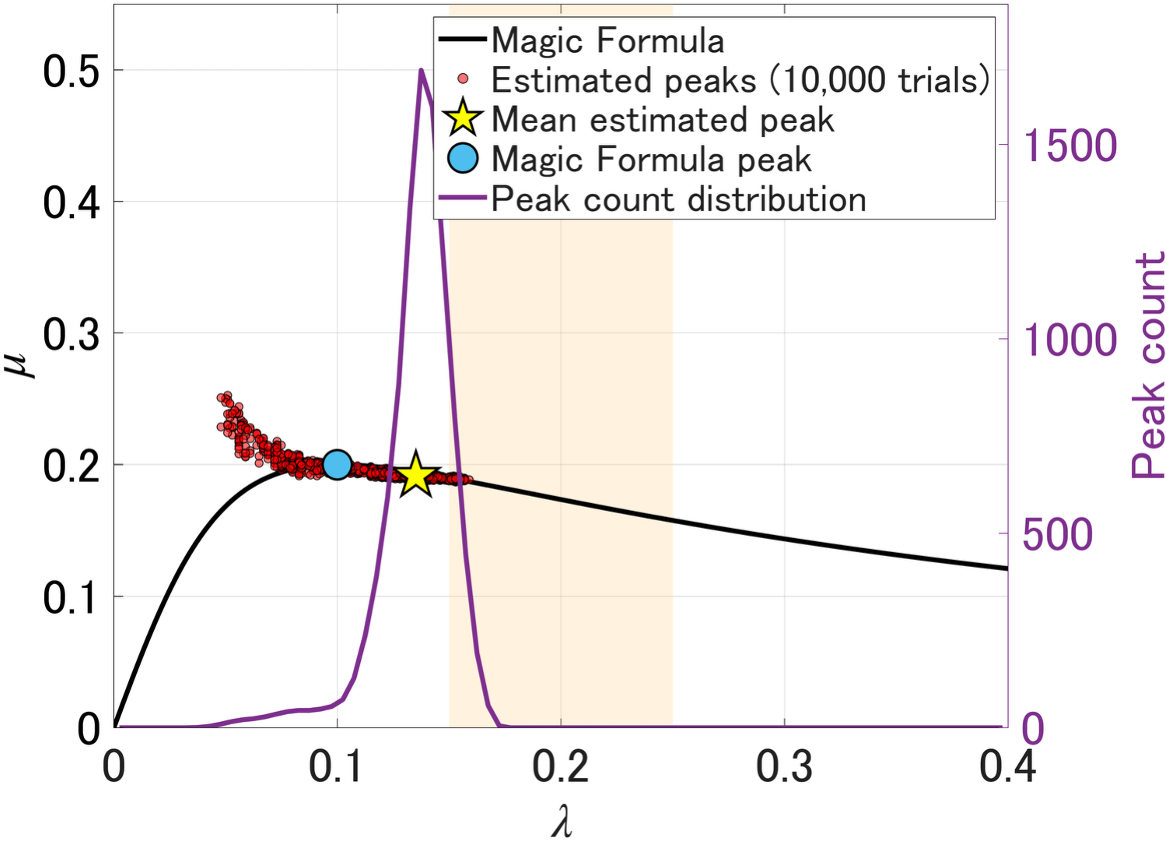
\includegraphics[width=\linewidth]{fig/5_road81_0.15_0.25_10000.png}
        \subcaption{路面2 / 観測範囲 : $0.15\le\lambda\le0.25$.}
        \label{fig:5_road81_0.15_0.25_10000}
    \end{minipage}
    \caption{10000回実行時の推定ピーク点分布.}
    \label{fig:5_result_10000}
\end{figure}

\section{シミュレーション上の走行データから取得した路面$\mu-\lambda$特性からの$\lambda_\mathrm{peak}$推定の検証}
\subsection{シミュレーション条件：スリップ率制御}
MATLAB/Simulinkを用いたシミュレーションにより, $\mu-\lambda$曲線の部分的な範囲のみの観測情報から, 曲線全体およびピーク点推定がどれほど精度で行われるかを検証した. 
データ取得は, スリップ率制御により, $0.0\le\lambda\le0.6$の範囲で上下させることで全体の特性を取得した. 
その上で, 適当な範囲を指定し, その中で200点の測定点をランダムに用いて推定を行った. 
検証は, 学習に用いていない2種類の路面に対し, 2種類の観測範囲($0.05\le\lambda\le0.15$, $0.15\le\lambda\le0.25$)で行った. 

\subsection{検証内容}
\subsubsection{1回推定実行時の推定曲線と推定ピーク点}
まず, 1度推定を行った際の推定曲線と推定ピーク点のグラフをFig.\ref{fig:5_result_curve}に示す. 
黒線が入力した路面モデルのMagic Formula曲線であり, 赤線が推定した$\mu-\lambda$曲線であるが, 単一のモデルを用いて複数の路面および観測範囲において一定精度の推定ができていることが読み取れる. 

\subsubsection{10000回実行時の推定ピーク点分布}
また, 同様の測定範囲で, 入力点パターンをランダムにし10000回推定を実行した際のピーク点分布をグラフをFig.\ref{fig:5_result_10000}に示す. 
黒線は先ほど同様路面モデルのMagic Formula曲線であり,赤点が推定した各ピーク点(合計10000点)である. また, 紫線は推定ピーク点の分布を表し, 対応する縦軸は右縦軸である. 
この結果より, ピーク付近の特性が取れていれば, 高い精度で推定ピーク点が真値のピーク付近に分布することがわかる.
また, ピーク付近の情報が得られていない(Fig.\ref{fig:5_road81_0.15_0.25_10000})場合は, 推定ピーク点が真のピークからズレたところに推定されているが, 観測範囲に対し$\lambda$が大小いずれの領域にいるかは高精度で判定できているため, オンライン推定の際に次ステップでよりピークに近い点の情報が得られ, 最終的に正しいピーク推定が行われると想定される.

%%================ 第6章 ================%%
\clearpage
\section{台上試験機を用いた実走行データから取得した路面$\mu-\lambda$特性からの$\lambda_\mathrm{peak}$推定の検証}
\subsection{実験条件}
実験は, 前述した台上試験機であるITHDを用いて行った. 
実験の様子をFig.\ref{fig:6_ithd}に示す.
\begin{figure}[tb]
    \centering
    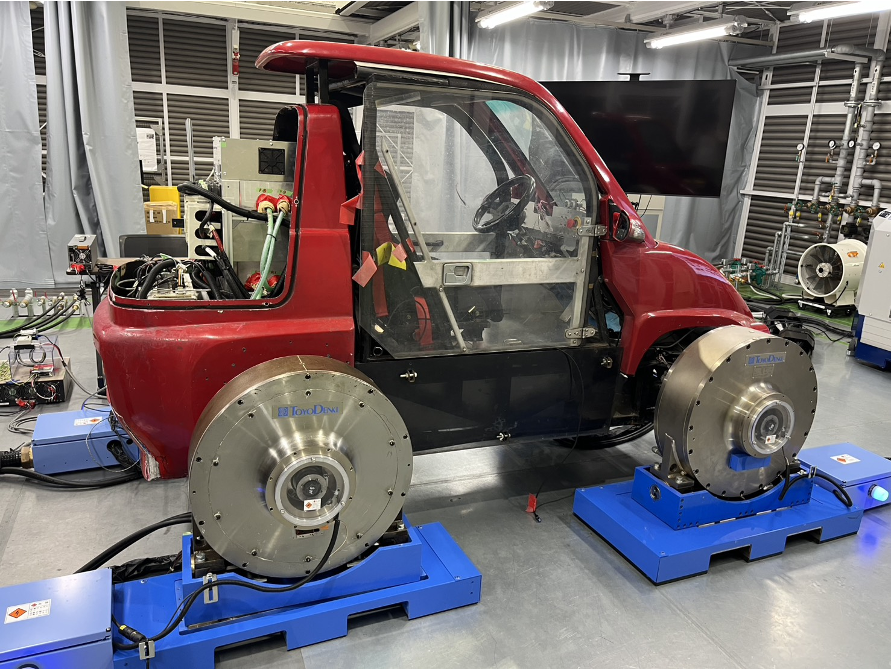
\includegraphics[width=0.4\linewidth]{fig/6_ithd.png}
    \caption{インタイヤハウスダイナモ(ITHD)の写真.}
    \label{fig:6_ithd}
\end{figure}
ITHDは自分が指定した路面モデルのMagic Formulaパラメータを入力することができ, これにより様々な種類の路面における走行を模擬することが可能である. 
これを用いて複数種類の路面における走行データを取得し, 様々な路面における$\mu-\lambda$曲線および最適スリップ率$\lambda_\mathrm{peak}$の推定精度を検証した. 


\subsection{実験内容}
\subsubsection{路面モデル}
今回の検証では, 2種類の低$\mu$路に関して, 対応するMagic FormulaパラメータをITHDに入力した. 
それぞれパラメータは, $(B,C,D,E) = (28.9, 1.91, 0.235, 0.810), (5.832, 2, 0.5, -0.8)$に設定した. 
学習時にはこの路面パラメータは入力していない. 

\subsubsection{制御内容}
低$\mu$路における$\mu-\lambda$特性を十分に取得するため, スリップ率制御により$0\le\lambda\le 0.3$の範囲に関し, 単調増加方向, 減少方向両方についてスリップ率を変動させた.
ただし, この際$V=0$からではスリップ率制御では発進できないため, 一定速度まで速度制御を行い, 速度が一定になった後にスリップ率制御に切り替えた.

\subsection{実験結果}
特性の異なる2種類の路面において得られた$\mu-\lambda$特性のうち, $0.15 \le \lambda \le 0.25$の範囲の200点のみが観測できた状況のみを仮定して, 推定曲線およびピーク点の精度を検証した. 
ここで, 200点としているのは, 実走行時のオンライン推定において使用するデータ点数を想定したものであり, サンプリング周波数は$\SI{1}{\kilo \hertz}$であるため, 0.2秒間のデータ点に対応する.

検証結果をFig.\ref{fig:6_curve_peak}およびFig.\ref{fig:6_10000peak}に示す. 

\begin{figure}[tb]
    \centering
    \begin{minipage}{0.4\linewidth}
        \centering
        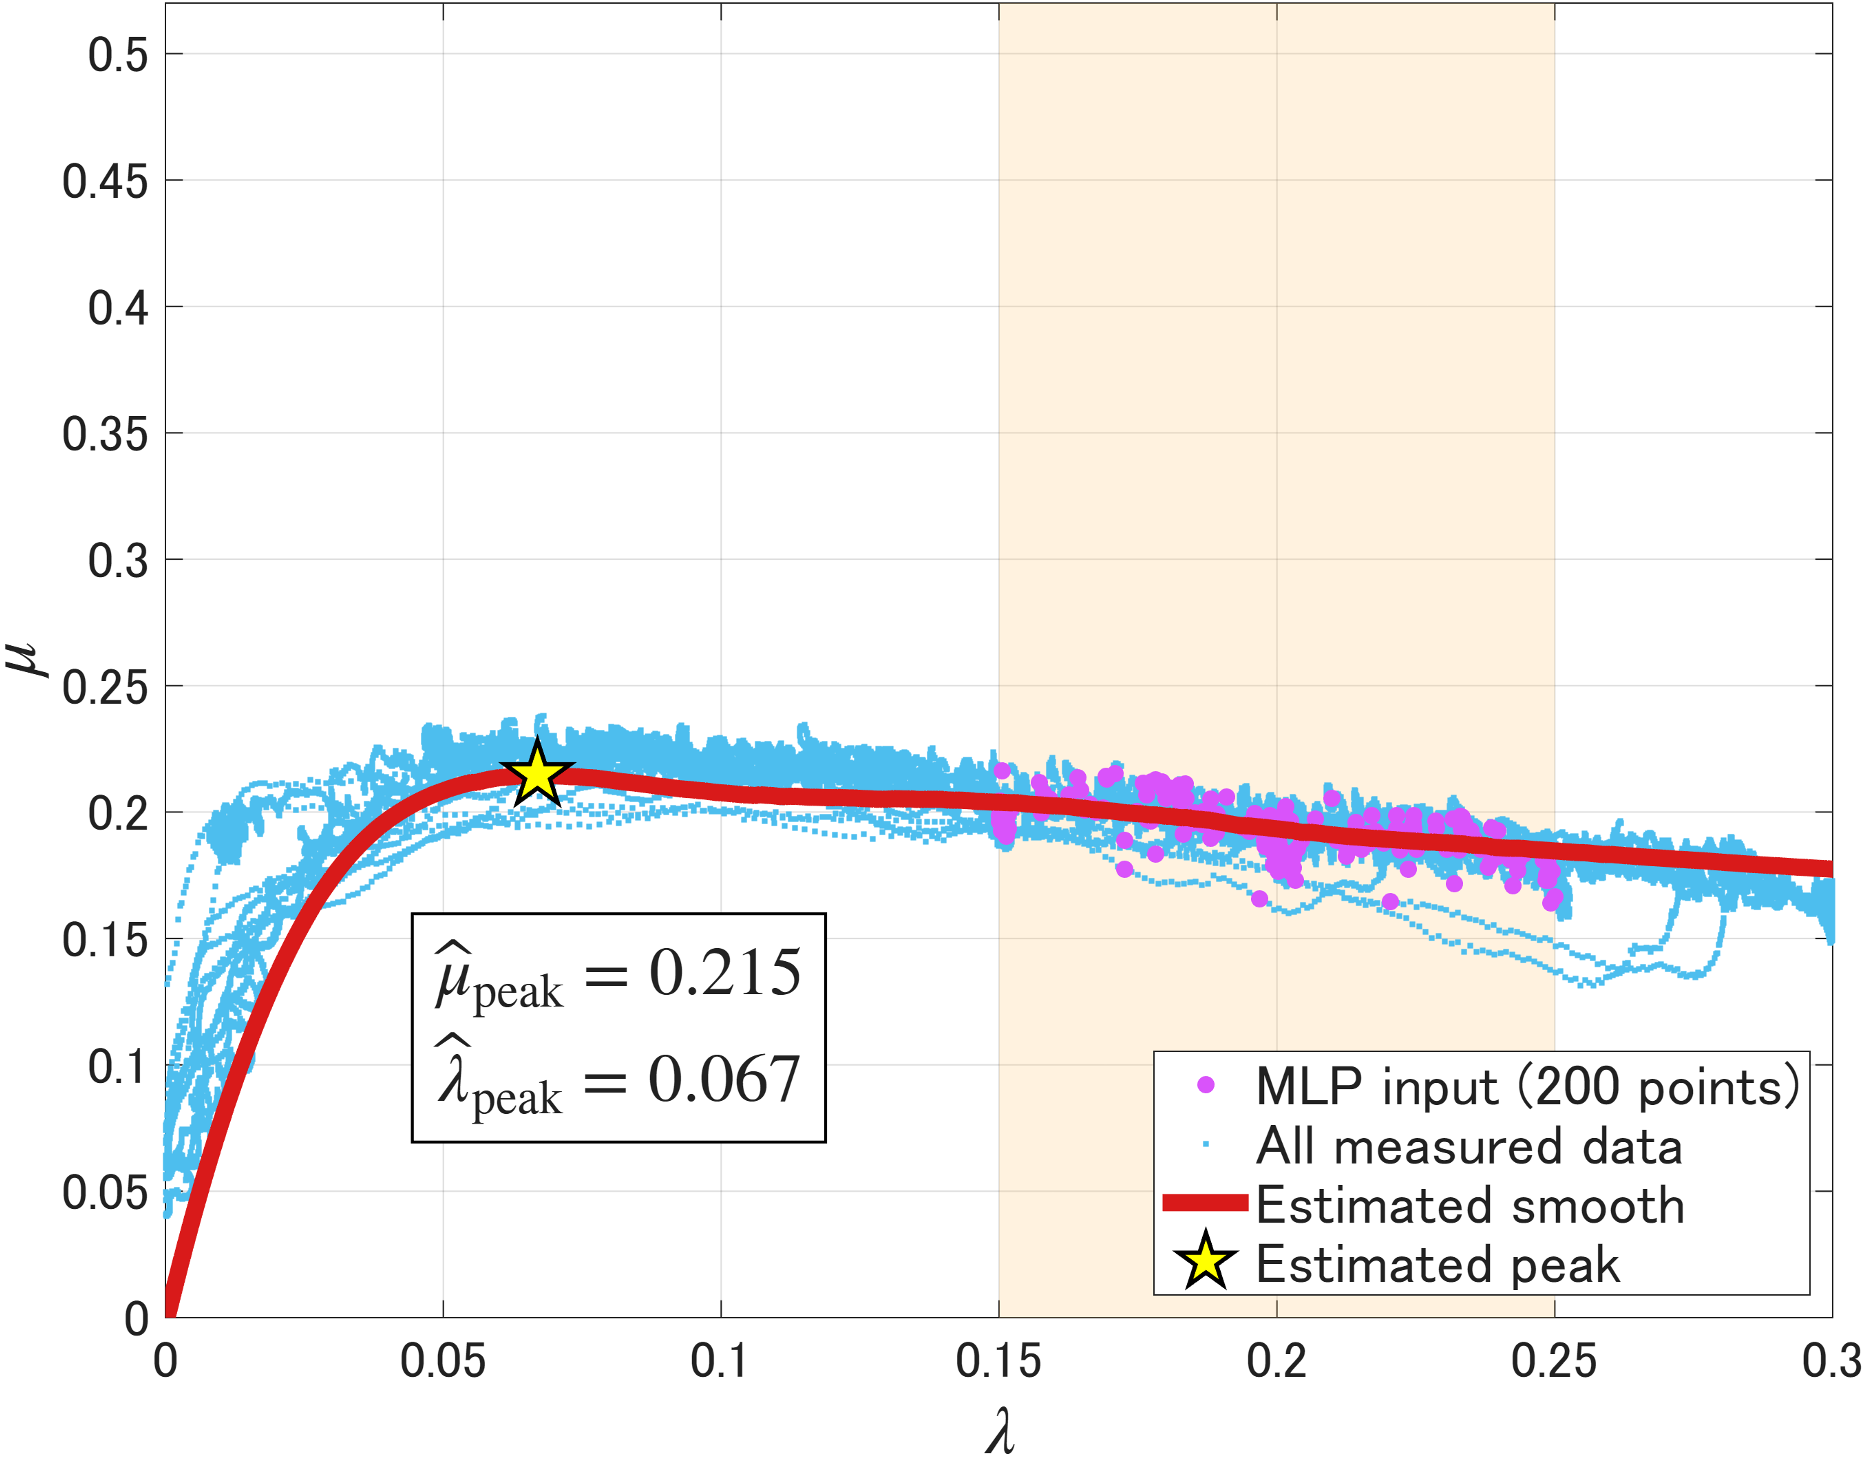
\includegraphics[width=\linewidth]{fig/6_curve_peak_7.png}
        \subcaption{$(B,C,D,E) = (28.9, 1.91, 0.235, 0.810)$の路面}
        \label{fig:6_curve_peak_7}
    \end{minipage}
    \hfill
    \begin{minipage}{0.4\linewidth}
        \centering
        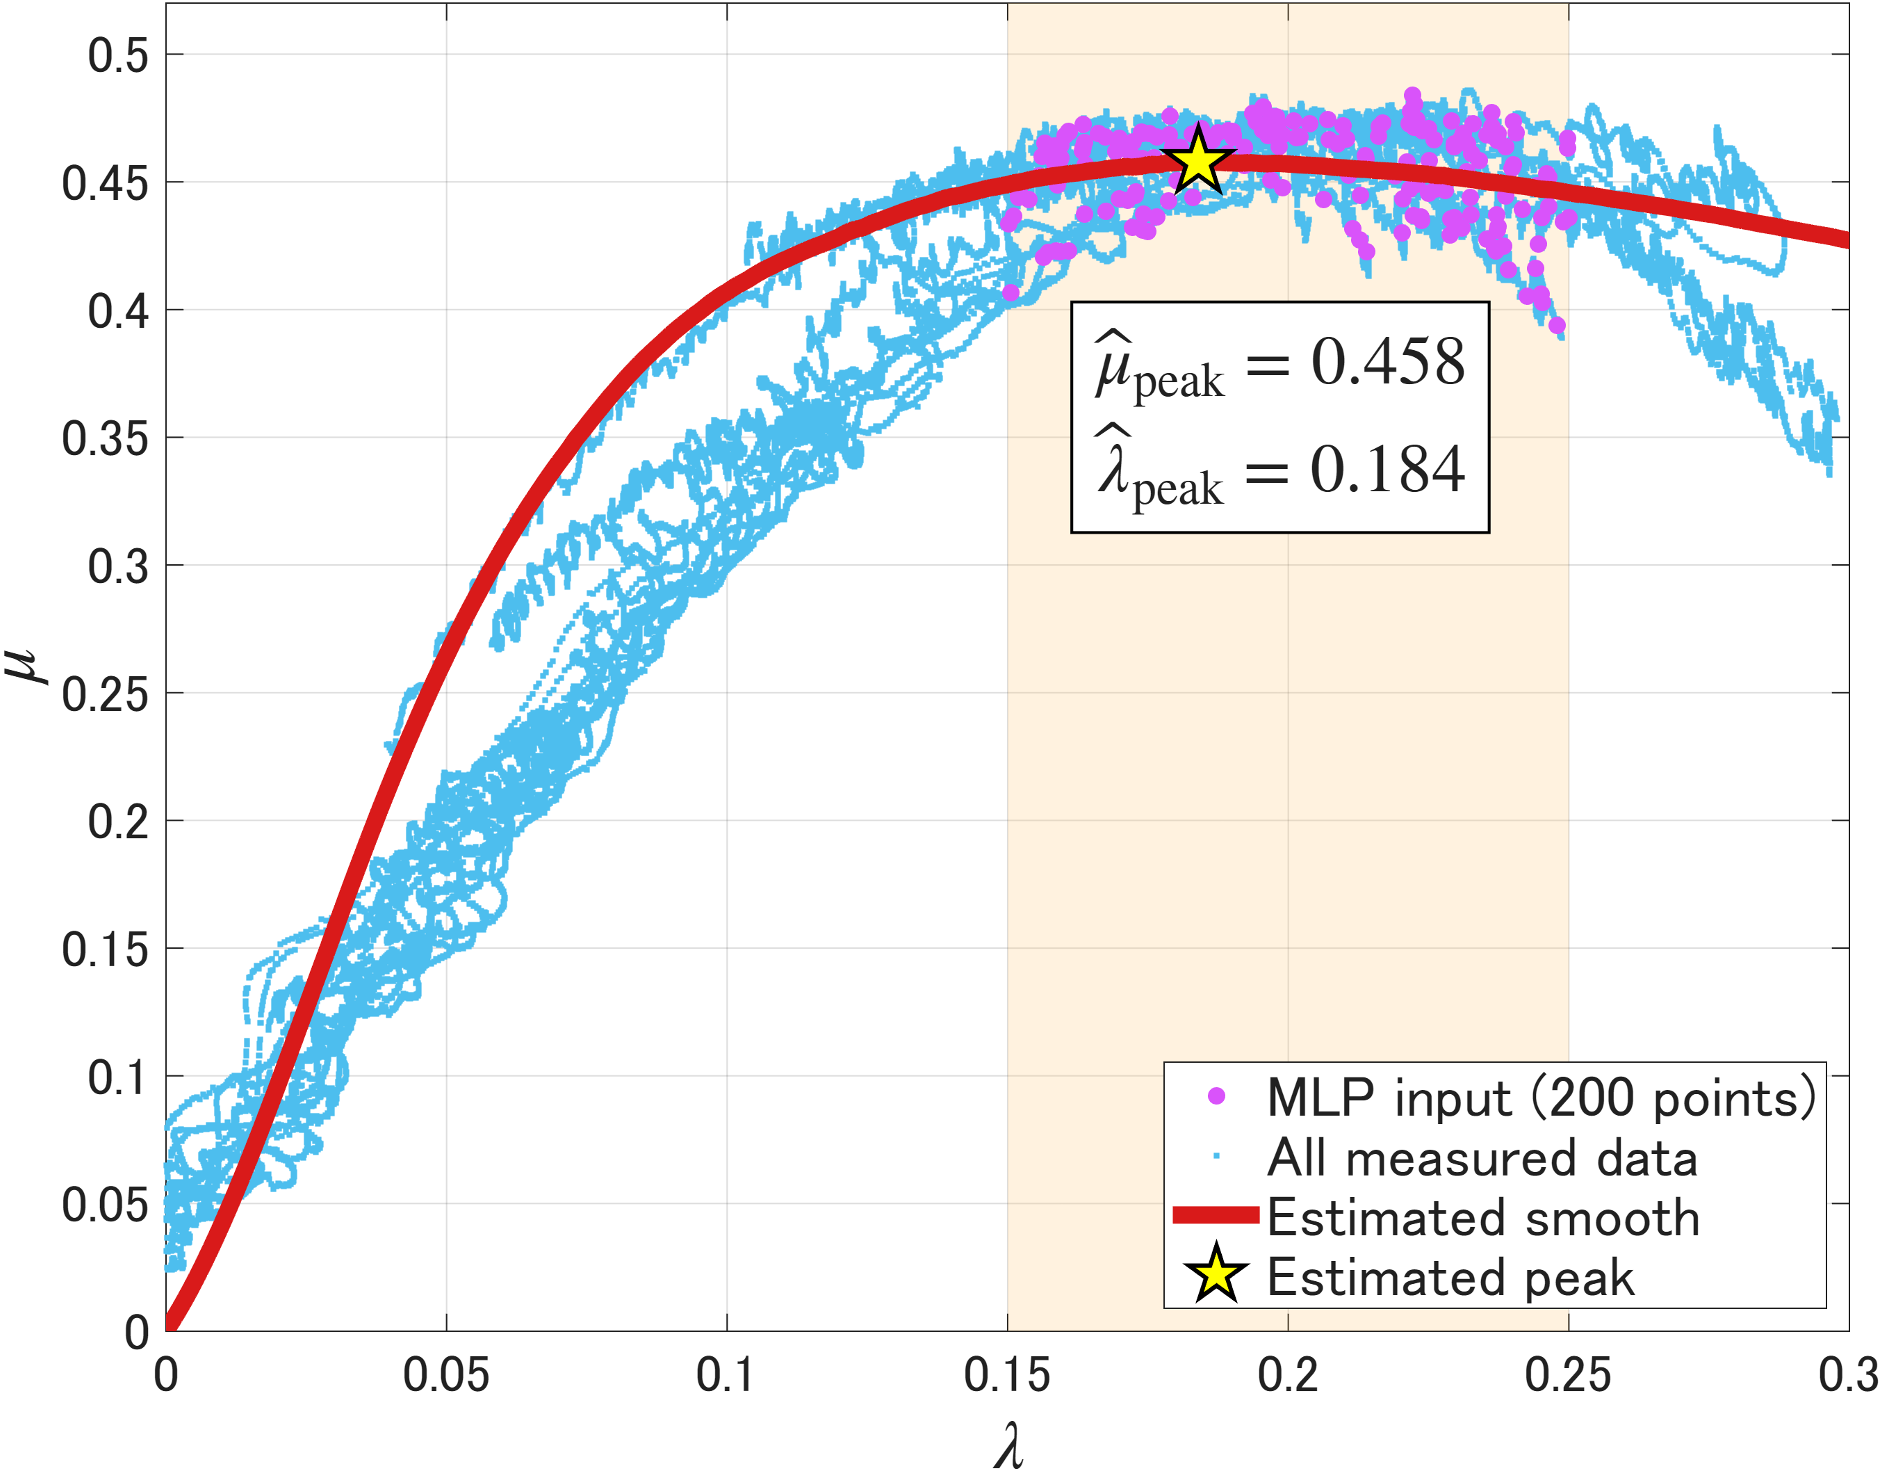
\includegraphics[width=\linewidth]{fig/6_curve_peak_4.png}
        \subcaption{$(B,C,D,E) = (5.832, 2, 0.5, -0.8)$の路面.}
        \label{fig:6_curve_peak_4}
    \end{minipage}
    \caption{推定$\mu-\lambda$曲線と推定ピーク点.}
    \label{fig:6_curve_peak}
\end{figure}

\begin{figure}[tb]
    \centering
    \begin{minipage}{0.4\linewidth}
        \centering
        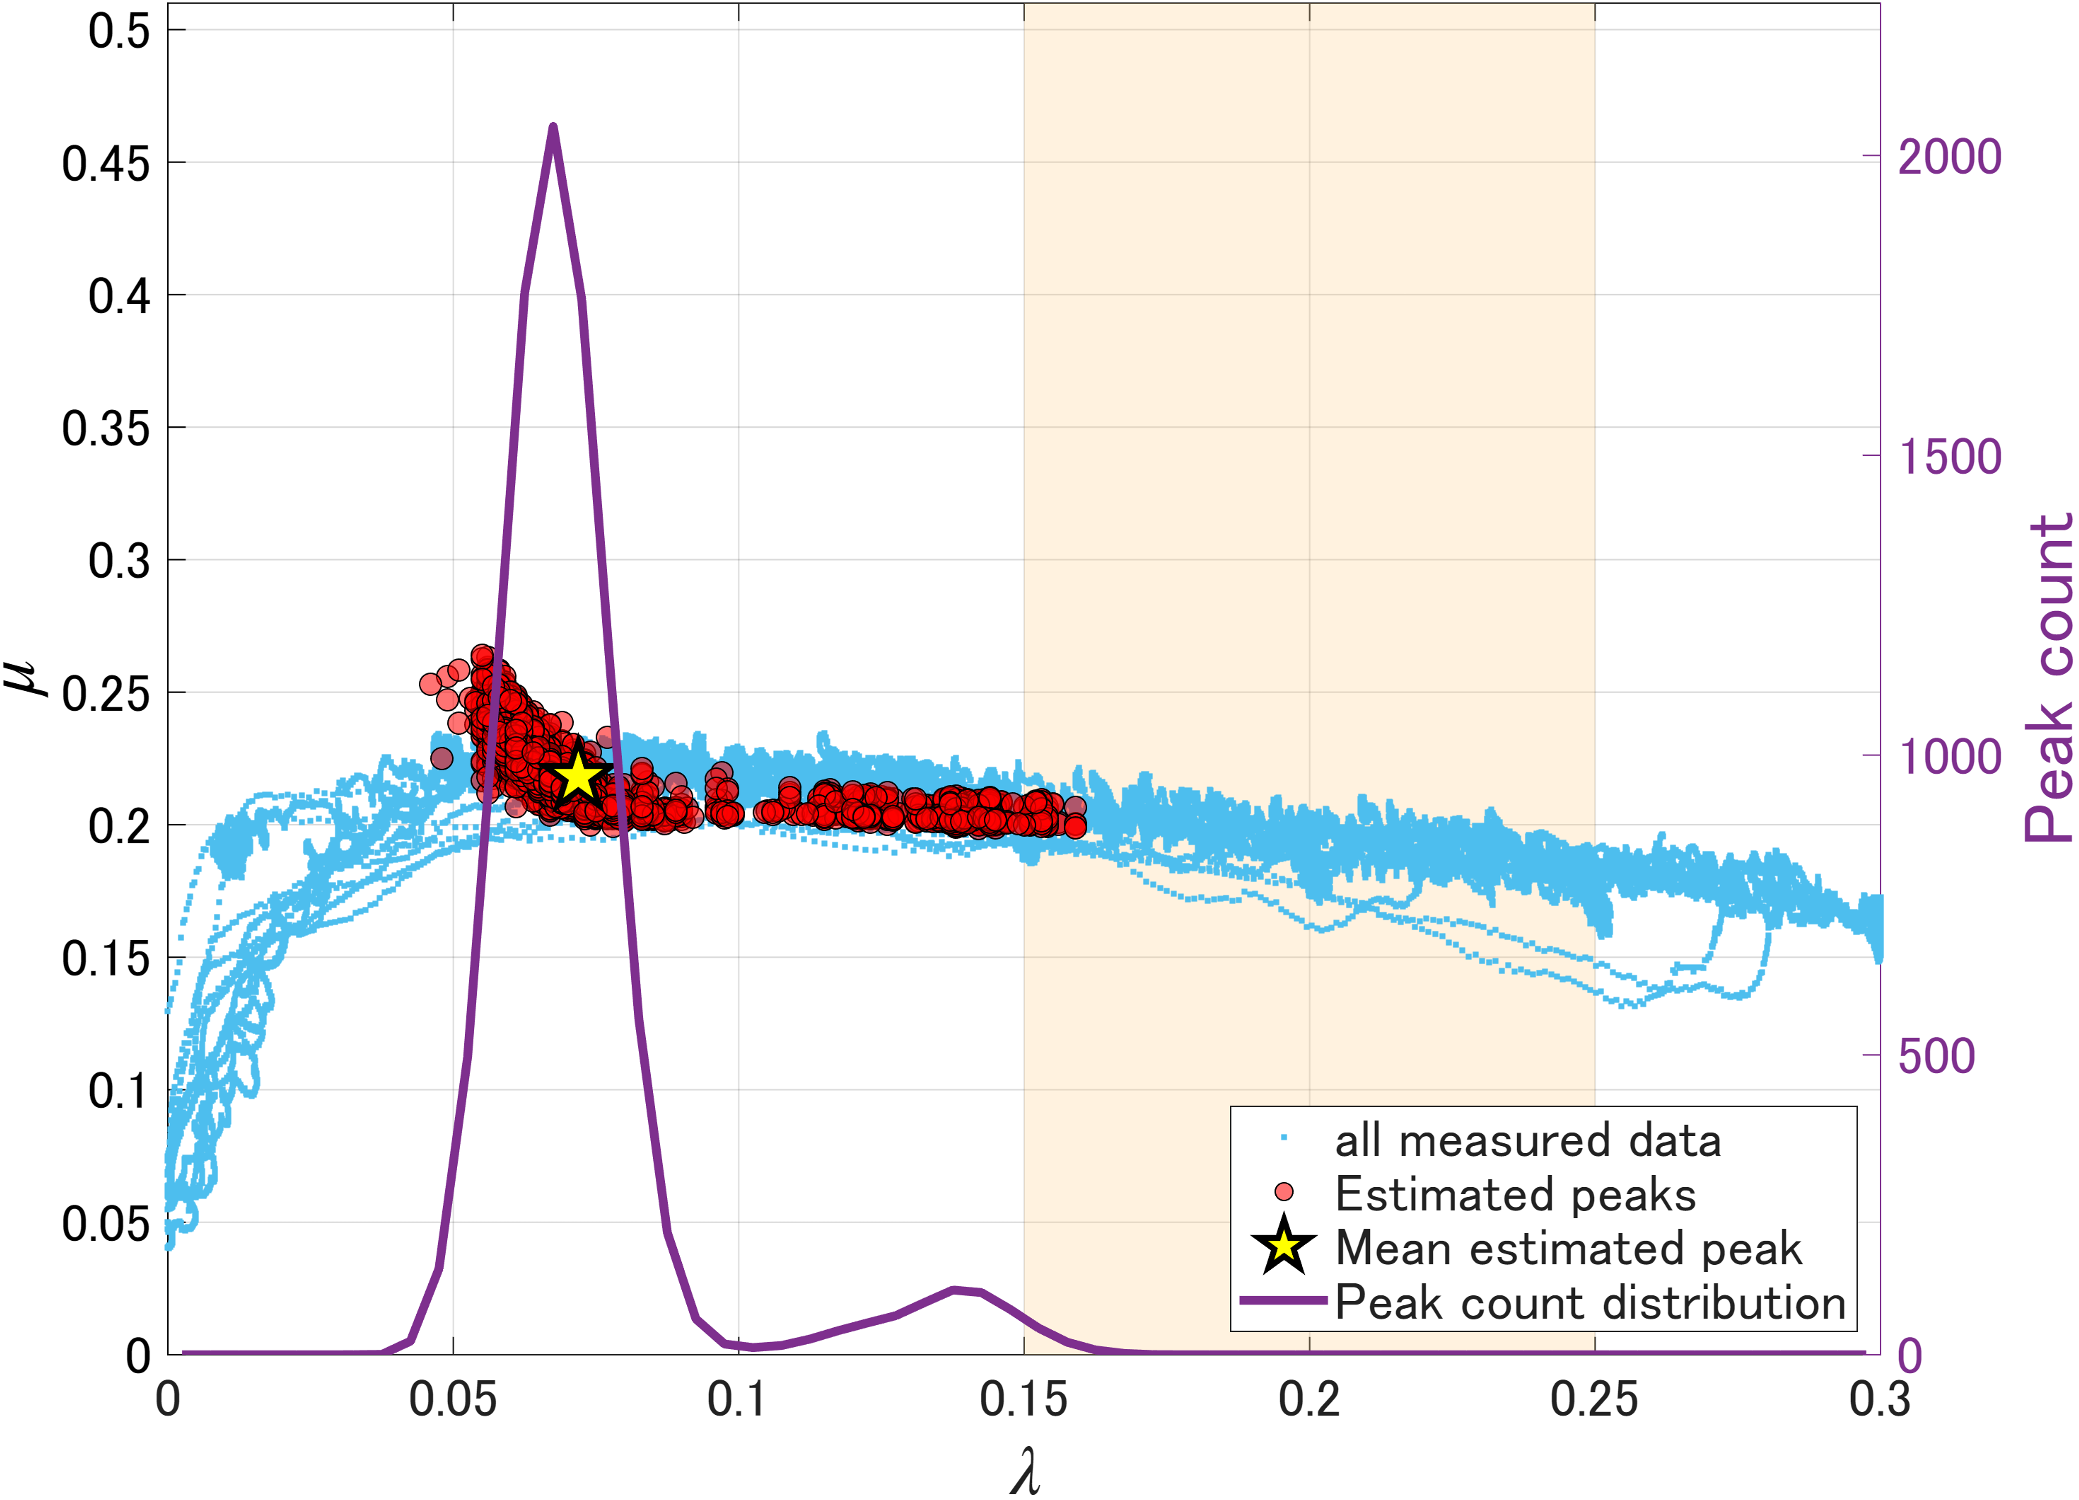
\includegraphics[width=\linewidth]{fig/6_10000peak_7.png}
        \subcaption{$(B,C,D,E) = (28.9, 1.91, 0.235, 0.810)$の路面}
        \label{fig:6_10000peak_7}
    \end{minipage}
    \hfill
    \begin{minipage}{0.4\linewidth}
        \centering
        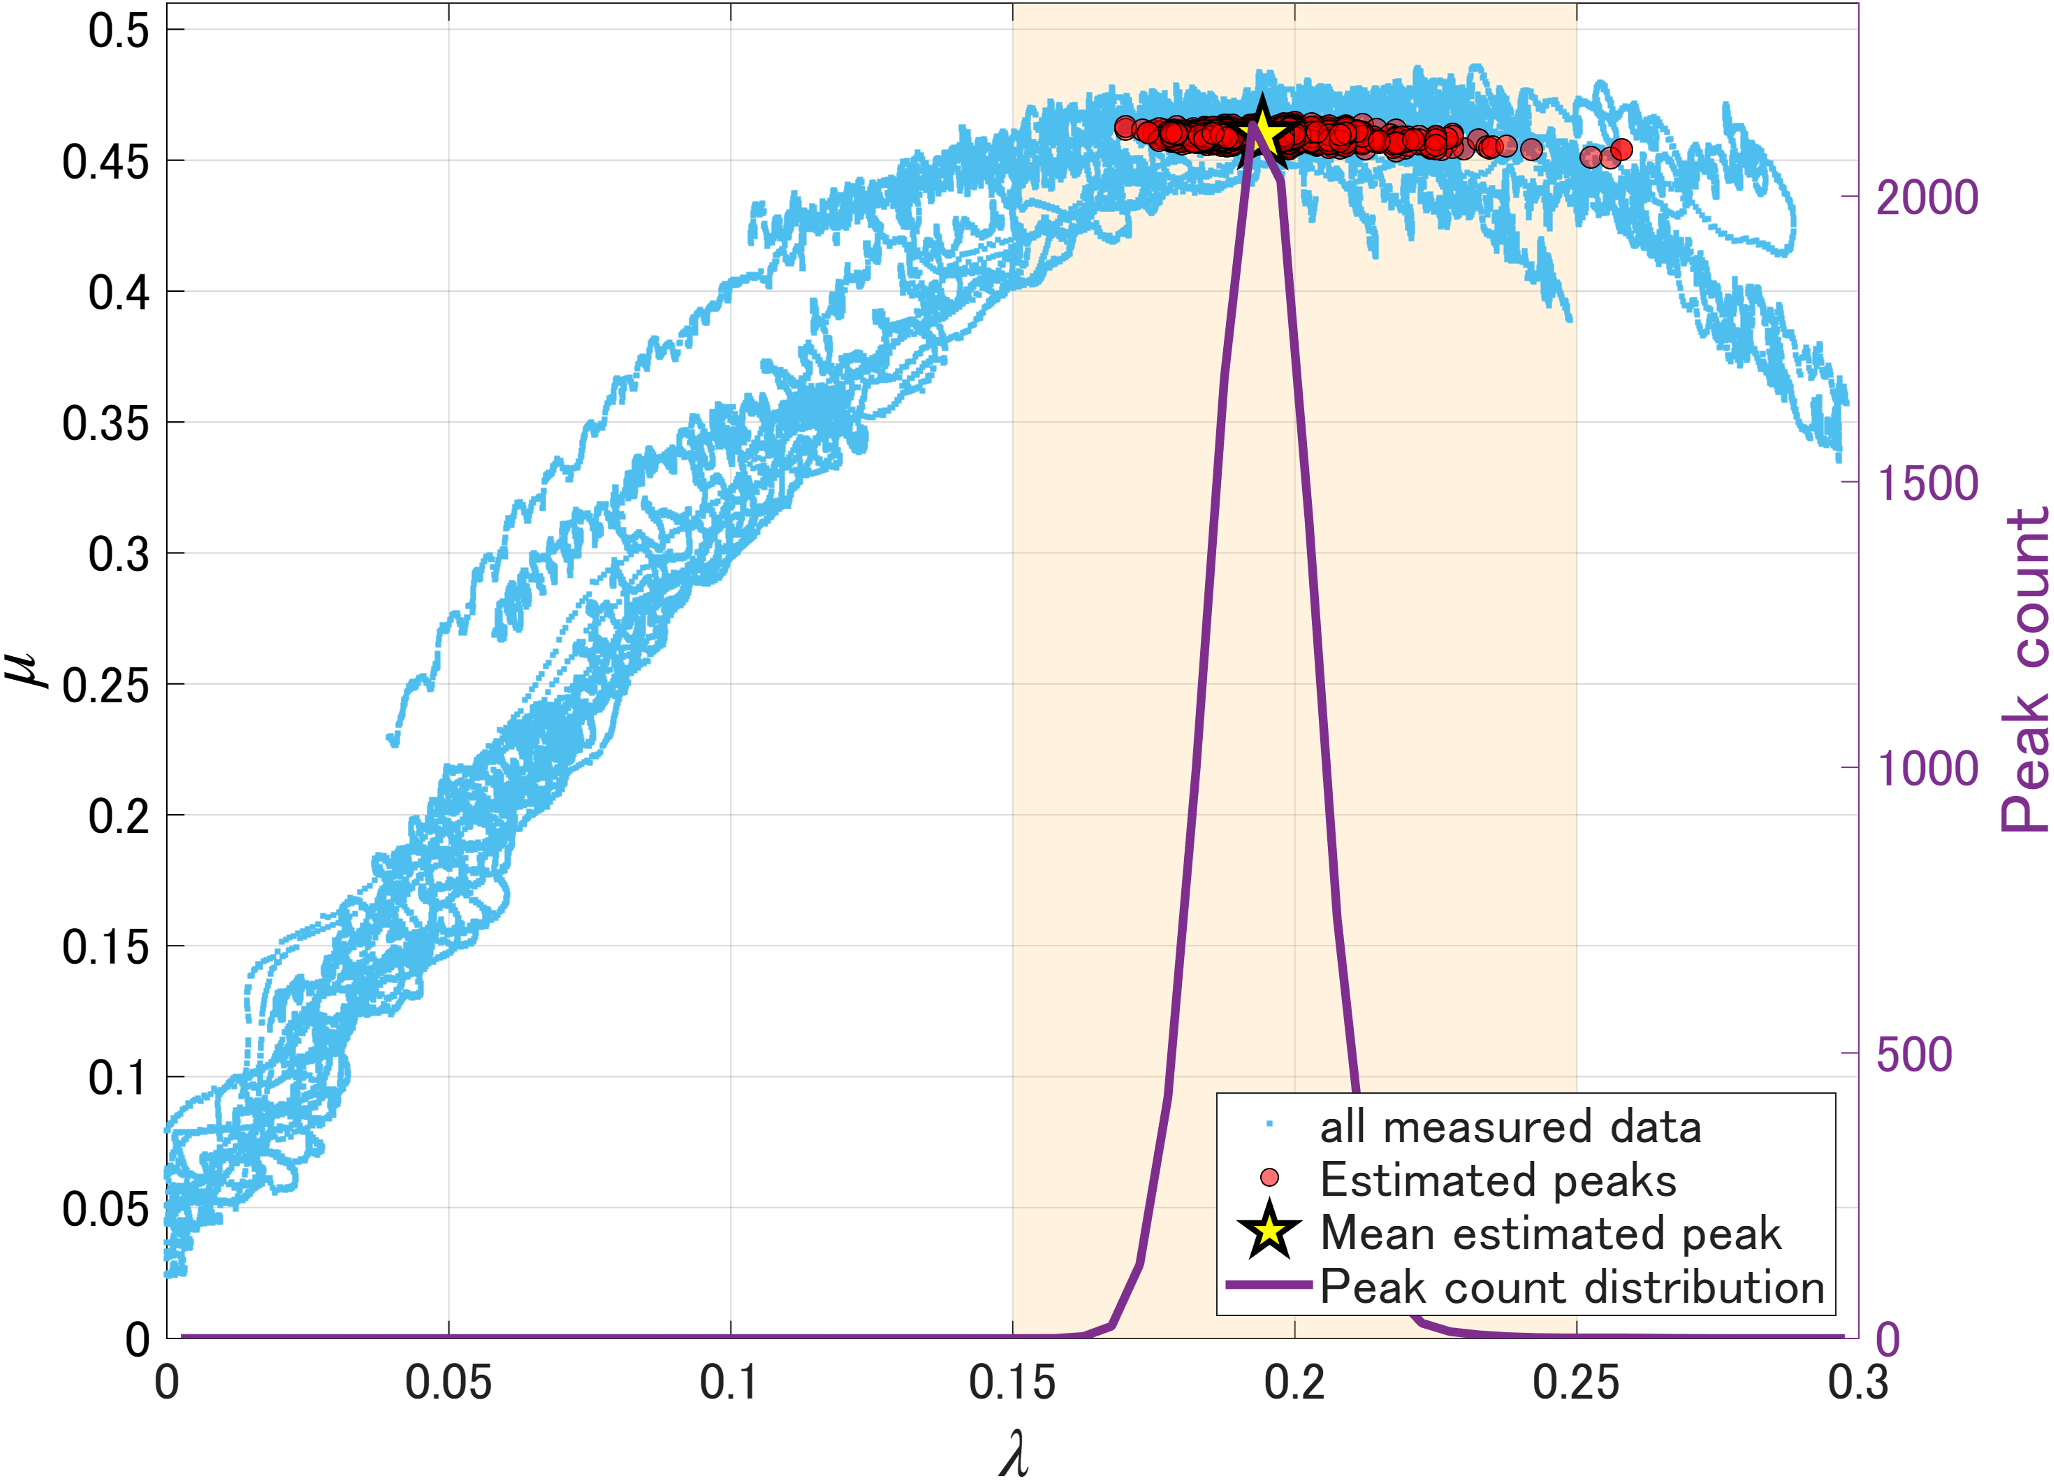
\includegraphics[width=\linewidth]{fig/6_10000peak_4.png}
        \subcaption{$(B,C,D,E) = (5.832, 2, 0.5, -0.8)$の路面.}
        \label{fig:6_10000peak_4}
    \end{minipage}
    \caption{10000回推定実行時のピーク点分布.}
    \label{fig:6_10000peak}
\end{figure}

Fig.\ref{fig:6_curve_peak}の水色の点は, スリップ率制御による実測点, ピンク色の点は推定に使用した入力点, 赤色の曲線は推定された$\mu-\lambda$曲線, 黄色の星は曲線から決定されたピーク点をそれぞれ表す. 
水色の点群のピーク付近に推定ピーク点が存在していれば, 精度の良い推定ができていると言える. 
Fig.\ref{fig:6_curve_peak_7}においては, ピーク付近の特性が取得できていないにも関わらず, 推定曲線が実測点の分布に追従しており, 推定ピーク点も妥当な値となっている. 
Fig.\ref{fig:6_curve_peak_4}においては, ピーク付近のデータが取得できており, ピーク判定が妥当に行われていることが読み取れる. 推定曲線は観測できていない領域においては若干精度は低下しているが, 大まかな傾向は掴んでいると言えるほか, ピーク以外の部分の追従精度はピーク判定には影響をもたらさないため大きな問題ではないと言える. 

続いて, Fig.\ref{fig:6_10000peak}は, 推定を10000回実行した結果である.
赤色の点は各推定実行時の推定ピーク点を示し, 黄色の星は全推定結果の平均値を示す. 
また, 紫色の曲線は推定ピーク点の分布を表す. 
この結果より, 10000回実行しても実測点のピーク付近に推定点が分布しており, Fig.\ref{fig:6_curve_peak}に示す結果が偶然出力されたデータでないことを裏付けるものになっている. 

%%================ 第7章 ================%%
\clearpage
\section{結論・今後の展望}
本研究では, 観測された$\mu-\lambda$プロットから$\mu-\lambda$曲線全体を推定することで最適スリップ率$\lambda_\mathrm{peak}$を推定することを目的としている. 
シミュレーションおよび実験を用いて, 提案した推定手法の有効性を検証した. 
その結果, オフライン検証において観測範囲を決定した際には, ピーク付近の情報が得られていなくとも一定程度妥当な$\lambda_\mathrm{peak}$が推定できることがわかった. 

今後の展望として, 実走行時におけるオンライン推定の実装を行いたいと考えている. 
そのためには, 測定範囲が狭い場合でもある程度妥当な推定を安定的に行うことができることを確認する必要があるほか, 妥当な推定ができていても推定結果が振動してしまう可能性があるため, その振動による車両振動を抑えるような工夫も施す必要があると考える. 

%%================ 参考文献 ================%%
\clearpage
\begin{thebibliography}{99}
        \bibitem{yoshimura}
        藤本 博志，吉村 雅貴：「電気自動車におけるスリップ率制御に基づく駆動力制御法」,自動車技術会春季学術講演会予稿集, No. 3-11, pp. 11--14, 2011.
        
        \bibitem{binhminh}
        B. M. Nguyen, Y. Hosomi, Y. Morimoto, T. Mizuguchi, and H. Fujimoto: “A Comprehensive History of Driving Force Control for Electric Vehicles,” IEEJ Journal of Industry Applications, Vol. 15, No. 2, pp. 173--186, 2025.
        
        \bibitem{zengin}
        N. Zengin, H. Zengin, B. Fidan, and A. Khajepour: “Slip Ratio Optimization in Vehicle Safety Control Systems Using Least-Squares Based Adaptive Extremum Seeking,” 2020 IEEE International Conference on Systems, Man, and Cybernetics (SMC), Toronto, ON, Canada, pp. 1445--1450, 2020.
        
        \bibitem{morimoto}
        Y. Morimoto, T. Mizuguchi, Y. Hosomi, B. M. Nguyen, and H. Fujimoto: “Proposal of Active Sensing Wheel Based Optimal Slip Ratio Estimation for In-Wheel Motor Vehicles,” IFAC-PapersOnLine, Vol. 59, No. 17, pp. 317--322, 2025.
        
        \bibitem{hannes}
        M. S. Heidfeld and R. Kasper: “UKF-Based State and Tire Slip Estimation for a 4WD Electric Vehicle,” Vehicle System Dynamics, Vol. 58, No. 10, pp. 1479--1496, 2020.
        
        \bibitem{pacejka}
        H. B. Pacejka and E. Bakker: “The Magic Formula Tyre Model,” Vehicle System Dynamics, Vol. 21, No. sup001, pp. 1--18, 1992.
        
        \bibitem{hori}
        Y. Hori: “Future Vehicle Driven by Electricity and Control-Research on Four-Wheel-Motored
        “UOT Electric March II”,”
        IEEE Transactions on Industrial Electronics, Vol. 51, No. 5, pp. 954--962, 2004.


        \bibitem{ithd}
        東洋電機製造株式会社: 「インタイヤハウスダイナモ（自動車用試験装置）」, 2025. [Online]. Available: \url{https://www.toyodenki.co.jp/product/automobile-test/} (accessed: 2026-09-29).
        

\end{thebibliography}

\end{document}
